\documentclass[11pt,a4paper]{article}

\usepackage[T1]{fontenc}
\usepackage{lmodern}
\usepackage[a4paper,margin=2.3cm]{geometry}
\usepackage{amsmath,amssymb}
\usepackage{booktabs}
\usepackage{float}
\usepackage{tabularx}
\usepackage{needspace}
\usepackage{array}
\usepackage{xcolor}
\usepackage{listings}
\usepackage{fancyhdr}
\usepackage{caption}
\usepackage{enumitem}
\usepackage{tikz}
\usetikzlibrary{arrows.meta,positioning}
\usepackage{pgfplots}
\pgfplotsset{compat=1.18}
\usepackage[hidelinks]{hyperref}

\newcommand{\rollno}{002410501045}

\pagestyle{fancy}
\fancyhf{}
\fancyhead[L]{Computer Networks, Project}
\fancyhead[R]{\rollno}
\fancyfoot[C]{\thepage}
\renewcommand{\headrulewidth}{0.4pt}

\captionsetup{font=small}
\captionsetup[lstlisting]{font=small,skip=4pt}
\setlist{itemsep=3pt,topsep=4pt}
\setlength{\emergencystretch}{3em}

\lstdefinelanguage{Rust}{
  morekeywords={as,break,const,continue,else,enum,false,fn,for,if,impl,in,let,loop,
    match,mod,move,mut,pub,ref,return,self,Self,static,struct,trait,true,type,use,
    where,while,Some,None,Ok,Err},
  sensitive=true,
  morecomment=[l]{//},
  morestring=[b]",
}
\lstset{
  language=Rust,
  basicstyle=\ttfamily\footnotesize,
  keywordstyle=\ttfamily,
  commentstyle=\color{gray}\itshape,
  numbers=left,
  numberstyle=\tiny\color{gray},
  numbersep=6pt,
  frame=single,
  rulecolor=\color{gray},
  xleftmargin=1.4em,
  framexleftmargin=1.4em,
  columns=fullflexible,
  keepspaces=true,
  showstringspaces=false,
  captionpos=t,
  aboveskip=8pt,
  belowskip=8pt,
}
\lstdefinestyle{plain}{numbers=none,xleftmargin=0pt,framexleftmargin=0pt,basicstyle=\ttfamily\scriptsize}

\begin{document}

% ---------------------------------------------------------------- title page
\begin{titlepage}
  \centering
  \vspace*{6cm}
  {\huge Computer Networks\par}
  \vspace{0.8cm}
  {\Large Project\par}
  \vspace{0.5cm}
  {\large BCSE III\par}
  \vspace{4cm}
  {\large Name: Abhirup Sarkar\par}
  \vspace{0.35cm}
  {\large Roll: \rollno\par}
  \vspace{0.35cm}
  {\large Group: A2\par}
  \vfill
\end{titlepage}
\setcounter{page}{1}

% ---------------------------------------------------------------- 1
\section{Problem Statement}

Implement network protocols in Rust, using only the standard library. The
first is a remote terminal. It was built first as a \emph{Telnet} server and
client (RFC~854), and then turned into an \emph{encrypted Telnet}, called
rsh: a server that gives an authenticated client a remote shell over an
encrypted TCP connection, together with a key generator and a file copy tool,
in the style of \texttt{ssh}, \texttt{ssh-keygen} and \texttt{scp}. All of
its cryptography (RSA, a digest, a stream cipher) is implemented from scratch.
The second protocol is the \emph{Address Resolution Protocol}: a server that
keeps an IP $\rightarrow$ MAC table and a client that resolves addresses and
caches the answers, exchanging packets in the RFC~826 format.

% ---------------------------------------------------------------- Telnet
% ---------------------------------------------------------------- Telnet
\section{Telnet}
\label{sec:telnet}

The remote shell in this project started as a Telnet server and client
(commit \texttt{4b08310}). Telnet showed how a remote terminal works, and also
why it cannot be used on a real network: everything it sends, passwords
included, can be read by anyone on the path. The rsh programs keep Telnet's
idea of a terminal session over TCP and add the missing security. This section
describes Telnet and the first implementation; Section~\ref{sec:rshdesign}
describes how it became rsh.

\subsection{The protocol}

Telnet is defined in RFC~854 (1983). A client opens a TCP connection to port
23 and both sides then exchange a stream of bytes in the format of the
\emph{Network Virtual Terminal} (NVT): 7-bit ASCII text, with every line ending
in \texttt{CR LF}. There are no packets or headers of Telnet's own; the
protocol lives entirely in the byte stream.

Control information is mixed into the data with an escape byte,
\texttt{IAC} (``interpret as command'', 255). The byte after \texttt{IAC} is a
command. A data byte that really is 255 is sent as \texttt{IAC IAC}.

\begin{table}[H]
\centering
\small
\begin{tabularx}{\textwidth}{@{}r p{3.4cm} X@{}}
\toprule
Code & Name & Meaning \\
\midrule
240 & \texttt{SE}   & end of a subnegotiation \\
241 & \texttt{NOP}  & no operation \\
242--249 & \texttt{DM BRK IP AO}\newline \texttt{AYT EC EL GA} & data mark, break, interrupt process, abort output, are you there, erase character, erase line, go ahead \\
250 & \texttt{SB}   & start of a subnegotiation: \texttt{IAC SB} \textit{option} \ldots\ \texttt{IAC SE} \\
251 & \texttt{WILL} & sender wants to enable an option on its side \\
252 & \texttt{WONT} & sender refuses to enable, or disables, an option on its side \\
253 & \texttt{DO}   & sender asks the other side to enable an option \\
254 & \texttt{DONT} & sender asks the other side not to use, or to stop, an option \\
255 & \texttt{IAC}  & interpret the next byte as a command; \texttt{IAC IAC} is a data byte 255 \\
\bottomrule
\end{tabularx}
\caption{Telnet commands (RFC 854).}
\end{table}

\textbf{Option negotiation} (RFC~855) lets the two ends agree on extra
features. Each option is a number, and a request takes three bytes, for
example \texttt{IAC DO 1} (``please echo''). The answer is either the
agreeing form (\texttt{WILL 1}) or the refusing form (\texttt{WONT 1}), and a
side must not answer a request for a state it is already in, which prevents
endless loops. Either side may always refuse, so a minimal implementation that
refuses everything still works with any client: both ends then fall back to
the plain NVT.

\begin{table}[H]
\centering
\small
\begin{tabular}{@{}r l l l@{}}
\toprule
Number & Option & RFC & Purpose \\
\midrule
0  & Binary transmission & 856  & send 8-bit data instead of NVT ASCII \\
1  & Echo                & 857  & the side that \texttt{WILL ECHO} echoes the characters it receives \\
3  & Suppress go-ahead   & 858  & full-duplex use, no \texttt{GA} after each turn \\
24 & Terminal type       & 1091 & the client names its terminal, e.g.\ \texttt{xterm} \\
31 & Window size (NAWS)  & 1073 & the client reports columns and rows \\
34 & Linemode            & 1184 & edit lines locally and send whole lines \\
\bottomrule
\end{tabular}
\caption{Common Telnet options.}
\end{table}

Telnet has no login protocol of its own. The server simply runs a
\texttt{login} program, which prints \texttt{login:} and \texttt{Password:} and
reads the answers from the same byte stream as everything else. Nothing is
encrypted, the server proves nothing about who it is, and the client proves
who it is only by typing a password across the network. For these reasons
Telnet was replaced by SSH, first released in 1995 and standardised in
RFC~4251--4254 (2006).

\subsection{Our Telnet implementation}

The first version (\texttt{telnet/}, about 260 lines of Rust, standard library only) had a
multi-threaded server on TCP port 2323 and an interactive client. Instead of a
real shell the server ran a small command interpreter with \texttt{help},
\texttt{echo <text>}, \texttt{time} and \texttt{quit}.

Both sides passed every received chunk through the same \texttt{Parser}, a
state machine that separates data bytes from \texttt{IAC} commands
(Figure~\ref{fig:telnetfsm}). It refuses every option, answering \texttt{DO}
with \texttt{WONT} and \texttt{WILL} with \texttt{DONT}, and skips
subnegotiations. Outgoing data goes through \texttt{escape}, which doubles each
255 byte.

\begin{figure}[H]
\centering
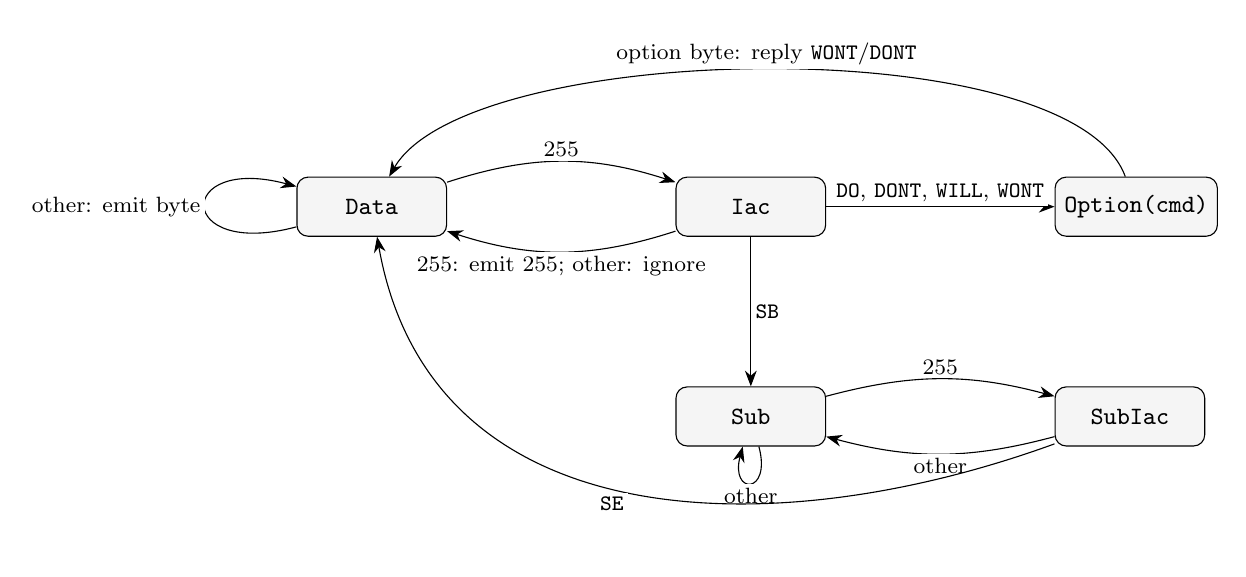
\begin{tikzpicture}[
  >={Stealth[length=2mm]}, node distance=2.1cm and 2.9cm, font=\small,
  st/.style={draw, rounded corners, minimum width=1.9cm, minimum height=0.75cm, fill=gray!8},
  lab/.style={font=\footnotesize, fill=white, inner sep=1.5pt},
]
  \node[st] (data) {\texttt{Data}};
  \node[st, right=of data] (iac) {\texttt{Iac}};
  \node[st, right=of iac] (opt) {\texttt{Option(cmd)}};
  \node[st, below=1.9cm of iac] (sub) {\texttt{Sub}};
  \node[st, right=of sub] (subiac) {\texttt{SubIac}};

  \draw[->] (data) to[loop left] node[lab, left]{other: emit byte} (data);
  \draw[->] (data) to[bend left=18] node[lab, above]{255} (iac);
  \draw[->] (iac) to[bend left=18] node[lab, below]{255: emit 255; other: ignore} (data);
  \draw[->] (iac) -- node[lab, above]{\texttt{DO}, \texttt{DONT}, \texttt{WILL}, \texttt{WONT}} (opt);
  \draw[->] (opt) to[out=110, in=60, looseness=0.55] node[lab, above]{option byte: reply \texttt{WONT}/\texttt{DONT}} (data);
  \draw[->] (iac) -- node[lab, right]{\texttt{SB}} (sub);
  \draw[->] (sub) to[loop below] node[lab, below]{other} (sub);
  \draw[->] (sub) to[bend left=15] node[lab, above]{255} (subiac);
  \draw[->] (subiac) to[bend left=15] node[lab, below]{other} (sub);
  \draw[->] (subiac) to[out=200, in=-80, looseness=1.1] node[lab, below left]{\texttt{SE}} (data);
\end{tikzpicture}
\caption{The Telnet input parser of the first version (\texttt{protocol.rs}).}
\label{fig:telnetfsm}
\end{figure}

\Needspace{16\baselineskip}
\begin{lstlisting}[caption={Option refusal and escaping in the Telnet parser (\texttt{protocol.rs}).}]
State::Iac => match b {
    IAC => { data.push(IAC); State::Data }           // IAC IAC is a data byte 255
    DO | DONT | WILL | WONT => State::Option(b),
    SB => State::Sub,
    _ => State::Data,                                  // NOP, GA, ...: ignored
},
State::Option(cmd) => {
    match cmd {
        DO => replies.extend([IAC, WONT, b]),          // "I will not"
        WILL => replies.extend([IAC, DONT, b]),        // "please do not"
        _ => {}                                        // WONT, DONT need no answer
    }
    State::Data
}
\end{lstlisting}

\subsection{A Telnet session on the wire}
\label{sec:telnetwire}

To show what Telnet exposes, the first version was rebuilt from the repository
history and a session was recorded through a TCP relay that copies every byte
(\texttt{report/tools/relay.py}). The client first sent three option requests
of the kind a Telnet client sends when it connects, then typed four lines. This is the complete
traffic, in order:

% generated by tools/gen_tables.py from data/ -- do not edit
\begin{lstlisting}[style=plain]
server -> client   63 B  "Welcome to the Rust telnet server\r\nType 'help' for commands\r\n> "
client -> server    9 B  ff fd 03 ff fb 18 ff fb 1f
                         = IAC DO SUPPRESS-GO-AHEAD, IAC WILL TERMINAL-TYPE, IAC WILL NAWS
server -> client    9 B  ff fc 03 ff fe 18 ff fe 1f
                         = IAC WONT SUPPRESS-GO-AHEAD, IAC DONT TERMINAL-TYPE, IAC DONT NAWS
client -> server   15 B  "login student\r\n"
server -> client   26 B  "Unknown command: login\r\n> "
client -> server   22 B  "echo my-password-123\r\n"
server -> client   19 B  "my-password-123\r\n> "
client -> server    6 B  "time\r\n"
server -> client   40 B  "Seconds since Unix epoch: 1794883707\r\n> "
client -> server    6 B  "quit\r\n"
server -> client    9 B  "Goodbye\r\n"
\end{lstlisting}


The server refused all three options, exactly as in
Figure~\ref{fig:telnetfsm}. Everything else is readable as it is. The line
that carried the ``password'' looks like this on the wire:

\begin{table}[H]
\centering
% generated by tools/gen_tables.py from data/ -- do not edit
{\setlength{\tabcolsep}{1.6pt}\footnotesize
\begin{tabular}{@{}lcccccccccccccccccccccc@{}}
\toprule
wire byte & \texttt{65} & \texttt{63} & \texttt{68} & \texttt{6f} & \texttt{20} & \texttt{6d} & \texttt{79} & \texttt{2d} & \texttt{70} & \texttt{61} & \texttt{73} & \texttt{73} & \texttt{77} & \texttt{6f} & \texttt{72} & \texttt{64} & \texttt{2d} & \texttt{31} & \texttt{32} & \texttt{33} & \texttt{0d} & \texttt{0a} \\
as text & \texttt{e} & \texttt{c} & \texttt{h} & \texttt{o} & \texttt{\textvisiblespace} & \texttt{m} & \texttt{y} & \texttt{-} & \texttt{p} & \texttt{a} & \texttt{s} & \texttt{s} & \texttt{w} & \texttt{o} & \texttt{r} & \texttt{d} & \texttt{-} & \texttt{1} & \texttt{2} & \texttt{3} & \texttt{\textbackslash r} & \texttt{\textbackslash n} \\
\bottomrule
\end{tabular}}

\caption{The bytes of \texttt{echo my-password-123} as captured: each byte is the ASCII code of the character typed.}
\label{tab:telnetpw}
\end{table}

Anyone who can see the packets (another host on the same Wi-Fi, a router, the
ISP) reads the password directly. They can also change the bytes or inject new
commands, and the client has no way to tell whether it is talking to the real
server at all.

\subsection{What an encrypted Telnet needs}

Turning Telnet into a safe remote shell needs four things that Telnet does not
have. Each became part of rsh:

\begin{enumerate}
\item \textbf{Server authentication}: the client must know it reached the right
  server. rsh gives each server an RSA host key and keeps a
  \texttt{known\_hosts} list.
\item \textbf{A shared secret}: both ends need a key that the observer does not
  have. The client makes a random session key and sends it encrypted with the
  host's public key.
\item \textbf{Confidentiality}: every byte after the key exchange is encrypted
  with a stream cipher keyed by the session key.
\item \textbf{Client authentication without a password on the wire}: the client
  signs the session key with its private key; the server checks the signature
  against \texttt{authorized\_keys}.
\end{enumerate}

\noindent A fifth requirement, \emph{integrity} (detecting changed bytes), is
not met by this version; Section~\ref{sec:cryptolimits} shows what that allows.


% ---------------------------------------------------------------- 2
\section{Design}

\subsection{What the programs are meant to do}

The repository holds two Cargo projects. \texttt{rsh/} is a workspace of four
crates and \texttt{arp/} is a single binary.

\textbf{rsh.} The server owns an RSA \emph{host key}. A client owns an
\emph{identity key}, made with \texttt{rsh-keygen}, whose public half must be
listed in the server's \texttt{authorized\_keys}. When a client connects, the
server first sends its host key. The client compares it with
\texttt{known\_hosts}: a new host is trusted and remembered, a host whose key
has changed is refused. The client then picks a random 32-byte \emph{session
key}, encrypts it with the host's public key and sends it, so that only the
server can read it. From that point both directions are encrypted with a
stream cipher keyed by the session key. The client proves who it is by signing
the session key and its user name with its private key.

After the handshake the client asks for one of three services. \texttt{Shell}
starts \texttt{cmd.exe} or \texttt{sh -i} on the server and streams its input
and output; \texttt{Upload} and \texttt{Download} move one file, which is how
\texttt{rcp} works. All keys and host files live in \texttt{\textasciitilde/.rsh/},
or in \texttt{\$RSH\_HOME}.

\textbf{arp.} Real ARP frames need raw Ethernet access, so the 28-byte ARP
packets are carried in UDP datagrams instead. The server answers a request for
an address in its table and, as real ARP does, learns the sender's IP and MAC
from every request it sees. The client derives its MAC from its IP
(\texttt{02:00:} followed by the four IP bytes), looks in its cache first, sends
a request on a miss and caches the reply for 60 seconds.

% ---------------------------------------------------------------- rsh as encrypted Telnet
\subsection{rsh: Telnet made secure}
\label{sec:rshdesign}

rsh does the job Telnet did, typing into a shell on another machine and seeing
its output, but it changes how the bytes are carried. Telnet mixes its control
commands into the data with \texttt{IAC}. rsh instead wraps everything in typed
messages inside length-prefixed frames, and encrypts the messages.
Table~\ref{tab:telnetvsrsh} compares the two point by point.

\begin{table}[H]
\centering
\footnotesize
\begin{tabularx}{\textwidth}{@{}l X X@{}}
\toprule
Concern & Telnet (RFC 854, our first version) & rsh \\
\midrule
Transport & TCP, port 23 (ours 2323) & TCP, port 2222 \\
Framing & none: one byte stream & 4-byte length + 1-byte message tag + fields \\
Control & \texttt{IAC} commands in the data, data 255 doubled & message types: \texttt{Shell}, \texttt{Eof}, \texttt{Exit}, \texttt{Disconnect}, \ldots \\
Feature agreement & option negotiation (\texttt{WILL}/\texttt{WONT}/\texttt{DO}/\texttt{DONT}) & none needed: one fixed protocol version \\
Server identity & none & RSA host key, checked against \texttt{known\_hosts} \\
Client login & name and password typed in clear (ours: no login) & signature with the client's private key, checked against \texttt{authorized\_keys} \\
Confidentiality & none & RSA key transport, then a stream cipher per direction \\
Integrity & none & none (Section~\ref{sec:cryptolimits}) \\
Remote side & NVT; ours a built-in command interpreter & a real shell process: \texttt{sh -i} or \texttt{cmd.exe} \\
Line endings & NVT \texttt{CR LF} & bytes passed through unchanged \\
End of session & TCP close & \texttt{Exit(code)}, then \texttt{Disconnect}; the client exits with the shell's code \\
File transfer & not part of Telnet (needs FTP) & \texttt{Upload} / \texttt{Download}, used by \texttt{rcp} \\
\bottomrule
\end{tabularx}
\caption{The first Telnet version compared with rsh.}
\label{tab:telnetvsrsh}
\end{table}

Figure~\ref{fig:layers} shows the two protocol stacks. rsh adds two layers
between TCP and the terminal data: framing, which keeps message boundaries, and
the cipher, which hides their content. Because the cipher sits under the message
layer, the rest of the program sends and receives plain \texttt{Message}
values and never handles encrypted bytes itself.

\begin{figure}[H]
\centering
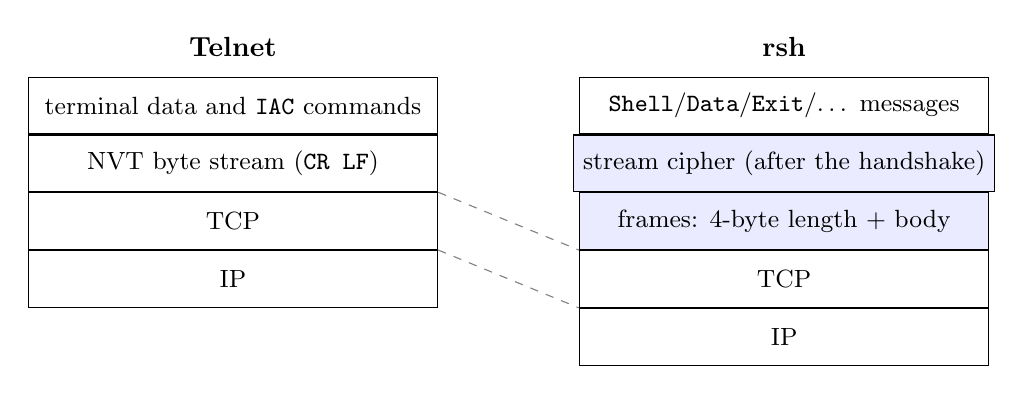
\begin{tikzpicture}[
  font=\small,
  lay/.style={draw, minimum width=5.2cm, minimum height=0.72cm, align=center},
  new/.style={lay, fill=blue!8},
]
  \node[font=\bfseries] at (0,0.75) {Telnet};
  \node[lay] (t3) at (0,0) {terminal data and \texttt{IAC} commands};
  \node[lay, below=0pt of t3] (t2) {NVT byte stream (\texttt{CR LF})};
  \node[lay, below=0pt of t2] (t1) {TCP};
  \node[lay, below=0pt of t1] (t0) {IP};

  \node[font=\bfseries] at (7,0.75) {rsh};
  \node[lay] (r4) at (7,0) {\texttt{Shell}/\texttt{Data}/\texttt{Exit}/\ldots\ messages};
  \node[new, below=0pt of r4] (r3) {stream cipher (after the handshake)};
  \node[new, below=0pt of r3] (r2) {frames: 4-byte length + body};
  \node[lay, below=0pt of r2] (r1) {TCP};
  \node[lay, below=0pt of r1] (r0) {IP};
  \draw[dashed, gray] (t1.north east) -- (r1.north west);
  \draw[dashed, gray] (t1.south east) -- (r1.south west);
\end{tikzpicture}
\caption{Protocol layers. The shaded layers are what rsh adds to a Telnet-style session.}
\label{fig:layers}
\end{figure}

A connection goes through three phases. The \emph{handshake}
(Figure~\ref{fig:handshake}) authenticates the server, sets up the session key
and authenticates the client. In the \emph{request} phase the client sends one
of \texttt{Shell}, \texttt{Upload}, \texttt{Download} or \texttt{Disconnect};
files can be moved several times on one connection. A \texttt{Shell} request
starts the \emph{interactive} phase, which lasts until the shell exits or
either side hangs up. Section~\ref{sec:rshsession} follows a real session
through all three phases, packet by packet.


\subsection{Cryptography in brief}

The RSA key uses two random 32-bit primes $p, q$, which gives a 64-bit modulus:
\[
  n = pq, \qquad e = 65537, \qquad ed \equiv 1 \pmod{(p-1)(q-1)}, \qquad
  c = m^{e} \bmod n, \qquad m = c^{d} \bmod n.
\]
Data is cut into 7-byte blocks, so that every block $m < 2^{56} < n$, and each
block becomes an 8-byte ciphertext. A signature is $s = H(x)^{d} \bmod n$ and is
checked with $s^{e} \equiv H(x) \pmod n$, where $H$ is a 64-bit digest built
from FNV-1a. Primes are found with the Miller--Rabin test using the first twelve
primes as witnesses, which is exact for every 64-bit number. The session cipher
is a \texttt{xoshiro256}-style generator seeded from the session key and a
direction label, so that client$\to$server and server$\to$client never share a
keystream. Figure~\ref{fig:handshake} shows the full exchange, and
Section~\ref{sec:crypto} explains every step with values from a recorded
session.

\begin{figure}[H]
\centering
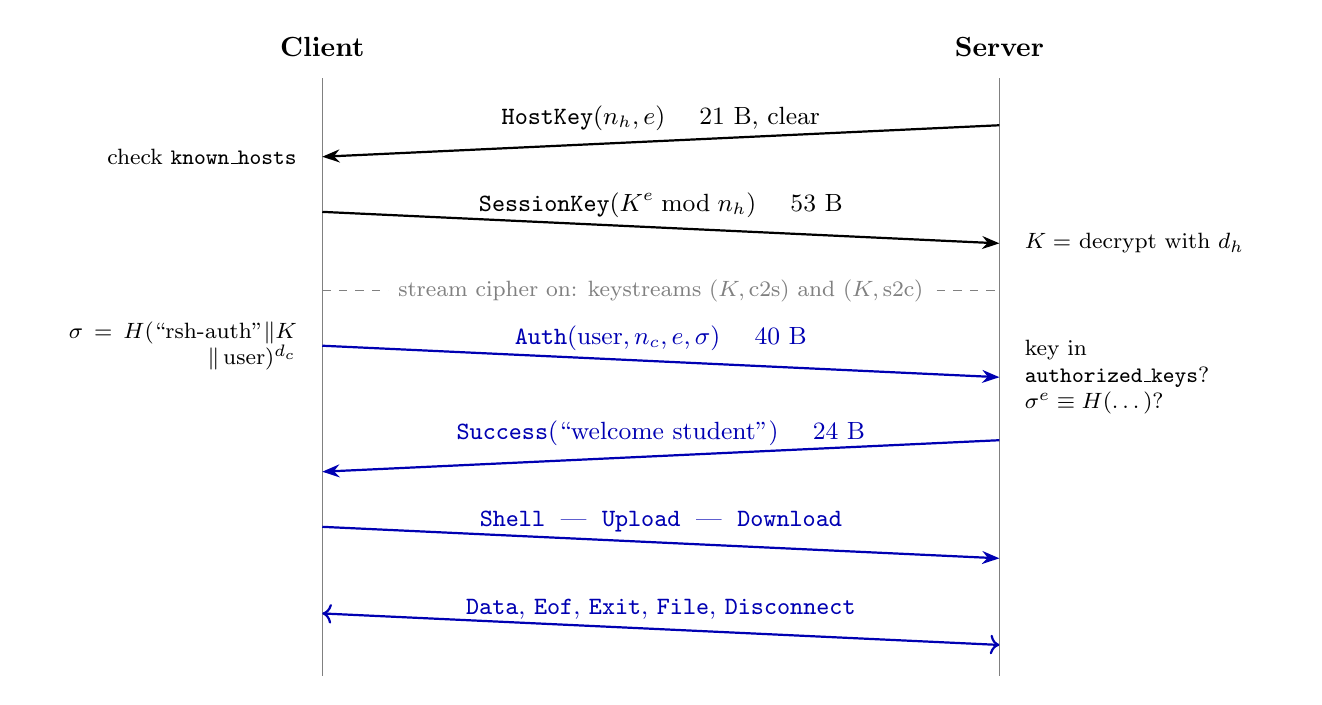
\begin{tikzpicture}[
  font=\small,
  msg/.style={-{Stealth[length=2.2mm]},thick},
  note/.style={font=\footnotesize,align=left,text width=3.3cm},
]
  \def\L{0} \def\R{8.6}
  \node[font=\bfseries] at (\L,0.4) {Client};
  \node[font=\bfseries] at (\R,0.4) {Server};
  \draw[gray] (\L,0) -- (\L,-7.6);
  \draw[gray] (\R,0) -- (\R,-7.6);

  \draw[msg] (\R,-0.6) -- node[above]{\texttt{HostKey}$(n_h, e)$ \quad 21 B, clear} (\L,-1.0);
  \node[note,anchor=east,align=right] at (\L-0.2,-1.0) {check \texttt{known\_hosts}};

  \draw[msg] (\L,-1.7) -- node[above]{\texttt{SessionKey}$(K^{e} \bmod n_h)$ \quad 53 B} (\R,-2.1);
  \node[note,anchor=west] at (\R+0.2,-2.1) {$K = $ decrypt with $d_h$};

  \draw[dashed,gray] (\L,-2.7) -- node[fill=white,font=\footnotesize]{stream cipher on: keystreams $(K,\text{c2s})$ and $(K,\text{s2c})$} (\R,-2.7);

  \draw[msg,blue!70!black] (\L,-3.4) -- node[above]{\texttt{Auth}$(\text{user}, n_c, e, \sigma)$ \quad 40 B} (\R,-3.8);
  \node[note,anchor=east,align=right] at (\L-0.2,-3.4) {$\sigma = H(\text{``rsh-auth''}\Vert K$\\$\Vert\,\text{user})^{d_c}$};
  \node[note,anchor=west] at (\R+0.2,-3.8) {key in\\ \texttt{authorized\_keys}?\\ $\sigma^{e} \equiv H(\dots)$?};

  \draw[msg,blue!70!black] (\R,-4.6) -- node[above]{\texttt{Success}(``welcome student'') \quad 24 B} (\L,-5.0);

  \draw[msg,blue!70!black] (\L,-5.7) -- node[above]{\texttt{Shell} \;|\; \texttt{Upload} \;|\; \texttt{Download}} (\R,-6.1);
  \draw[msg,blue!70!black,<->] (\L,-6.8) -- node[above]{\texttt{Data}, \texttt{Eof}, \texttt{Exit}, \texttt{File}, \texttt{Disconnect}} (\R,-7.2);
\end{tikzpicture}
\caption{The rsh handshake. Black messages travel in clear, blue ones are encrypted. Sizes are whole TCP frames measured in Section~\ref{sec:wire}.}
\label{fig:handshake}
\end{figure}

\subsection{Module structure}

\begin{table}[H]
\centering
\footnotesize
\begin{tabularx}{\textwidth}{@{}>{\ttfamily}l X@{}}
\toprule
\normalfont File & Contents \\
\midrule
rsh-crypto/src/math.rs      & modular multiply, power, gcd and inverse (128-bit intermediates) \\
rsh-crypto/src/prime.rs     & Miller--Rabin test and random prime generation \\
rsh-crypto/src/rsa.rs       & key generation, block encrypt/decrypt, sign/verify, fingerprint \\
rsh-crypto/src/cipher.rs    & stream cipher for the session \\
rsh-crypto/src/hash.rs      & FNV-1a based 64-bit digest \\
rsh-crypto/src/keyfile.rs   & text key file format, load and save \\
rsh-main/src/packet.rs      & 4-byte length-prefixed framing over TCP (max 64 MiB) \\
rsh-main/src/codec.rs, message.rs & typed message encoding and checked decoding \\
rsh-main/src/transport.rs   & encrypted send and receive, split into sender and receiver \\
rsh-main/src/handshake.rs   & host key, session key and authentication \\
rsh-main/src/server/        & listener, session loop, shell streaming, \texttt{cmd} echo filter, files \\
rsh-main/src/client/        & connecting, terminal $\leftrightarrow$ remote shell streaming \\
rsh-keygen/src/, rcp/src/   & key generator and file copy tool \\
arp/src/packet.rs           & ARP packet encoding and decoding \\
arp/src/server.rs, client.rs, cache.rs & UDP server with table, interactive resolver, cache with expiry \\
\midrule
rsh-crypto/tests/*.rs       & new: arithmetic, RSA, cipher, key files; factoring attack \\
rsh-main/tests/protocol.rs  & new: messages, frames, handshakes over TCP through a recording relay \\
arp/tests/arp.rs            & new: black-box tests of the \texttt{arp} binary with hand-built packets \\
\bottomrule
\end{tabularx}
\caption{Files of the two projects.}
\end{table}

\subsection{Wire formats}

Every rsh message is one frame: a 4-byte big-endian length, then a 1-byte tag
and the fields. Integers are big-endian \texttt{u64}; strings and byte arrays
carry a 4-byte length. Once the cipher is on, everything after the length is
encrypted.

\begin{table}[H]
\centering
\small
\begin{tabular}{@{}r >{\ttfamily}l l l@{}}
\toprule
Tag & \normalfont Message & Direction & Fields \\
\midrule
1  & HostKey     & server $\to$ client & $n$, $e$ \\
2  & SessionKey  & client $\to$ server & RSA ciphertext of $K$ \\
3  & Auth        & client $\to$ server & user, $n$, $e$, signature \\
4, 5 & Success, Failure & either      & text \\
6  & Shell       & client $\to$ server & -- \\
7, 8 & Data, Eof & both                & bytes / -- \\
9  & Exit        & server $\to$ client & exit code \\
10 & Upload      & client $\to$ server & remote path, file name, bytes \\
11, 12 & Download, File & client $\to$ server, back & path / name, bytes \\
13 & Disconnect  & client $\to$ server & -- \\
\bottomrule
\end{tabular}
\caption{rsh messages.}
\end{table}

\begin{table}[H]
\centering
\small
\begin{tabular}{@{}l l l l@{}}
\toprule
Bytes & Field & Value here & Meaning \\
\midrule
0--1   & htype & \texttt{00 01} & Ethernet \\
2--3   & ptype & \texttt{08 00} & IPv4 \\
4, 5   & hlen, plen & \texttt{06}, \texttt{04} & MAC and IP lengths \\
6--7   & oper  & \texttt{00 01} / \texttt{00 02} & request / reply \\
8--13  & sender hardware address & & MAC of the sender \\
14--17 & sender protocol address & & IP of the sender \\
18--23 & target hardware address & zero in a request & \\
24--27 & target protocol address & & IP being asked about \\
\bottomrule
\end{tabular}
\caption{The 28-byte ARP packet (RFC 826), sent as one UDP datagram.}
\end{table}

\subsection{Build and run}

\begin{lstlisting}[style=plain]
cd rsh && cargo build --release
target/release/rsh-keygen -a                      # make id_rsh and authorize it on this machine
target/release/rsh server [port]                  # default port 2222
target/release/rsh connect <host> [port]
target/release/rcp [-P port] <file> <host>:<remote-path>
target/release/rcp [-P port] <host>:<remote-path> <local-path>
cargo test --workspace

cd arp && cargo run -- server [port]              # default UDP port 4000
cargo run -- client [my-ip] [server] [port]       # input: an IPv4 address | cache | quit
cargo test
\end{lstlisting}

% ---------------------------------------------------------------- cryptography
% ---------------------------------------------------------------- Cryptographic implementation
\section{Cryptographic Implementation}
\label{sec:crypto}

All cryptography is written from scratch in the \texttt{rsh-crypto} crate,
about 410 lines with no dependencies. This section explains each part and then
follows one real recorded session byte by byte. The worked values come from a
session between the real \texttt{rsh} server and client, recorded through the
TCP relay of Section~\ref{sec:telnetwire} and decoded afterwards with the
server's private key (\texttt{report/tools/decoder}). Every table in
Sections~\ref{sec:hostkey}--\ref{sec:packets} is generated from that recording
(\texttt{report/data/}), and every value was checked by the decoder against the
library code itself.

\begin{table}[H]
\centering
\footnotesize
\begin{tabularx}{\textwidth}{@{}l l X@{}}
\toprule
Building block & File & Used for \\
\midrule
Modular arithmetic & \texttt{math.rs} & $a b \bmod m$, $a^{k} \bmod m$, $a^{-1} \bmod m$ on 64-bit numbers \\
Random numbers & \texttt{random.rs} & candidate primes, the 32-byte session key \\
Miller--Rabin & \texttt{prime.rs} & testing candidate primes \\
RSA, 64-bit modulus & \texttt{rsa.rs} & sending the session key; signing the login \\
Digest $H$ (FNV-1a) & \texttt{hash.rs} & the value that is signed; key fingerprints \\
Stream cipher & \texttt{cipher.rs} & encrypting every message after the key exchange \\
Key files & \texttt{keyfile.rs} & \texttt{id\_rsh}, \texttt{host\_key}, \texttt{authorized\_keys}, \texttt{known\_hosts} \\
\bottomrule
\end{tabularx}
\caption{The cryptographic building blocks.}
\end{table}

RSA is slow and works only on numbers smaller than $n$, so it is used twice per
connection: once to send the session key and once to sign the login. All the
terminal traffic is then encrypted with the fast stream cipher. Real SSH divides
the work the same way: public-key operations only to agree on a key and to
authenticate, a symmetric cipher for the data.

% ................................................................
\subsection{Modular arithmetic}

Every RSA operation is arithmetic modulo $n < 2^{64}$. The product of two such
numbers needs up to 128 bits, so \texttt{mul\_mod} widens to \texttt{u128}
before reducing:
\[
  \texttt{mul\_mod}(a, b, m) = (a \cdot b) \bmod m, \qquad a, b < m < 2^{64}, \quad a \cdot b < 2^{128}.
\]
\texttt{pow\_mod} computes $b^{k} \bmod m$ by \emph{square and multiply}. It
reads the exponent bit by bit from the lowest bit up: the base is squared at
every step and multiplied into the result where the bit is 1. A 64-bit exponent
therefore costs at most 64 squarings and 64 multiplications, instead of $k$
multiplications. \texttt{inv\_mod} finds $a^{-1} \bmod m$ with the extended
Euclidean algorithm, which keeps $s$ such that $\mathit{old\_r} \equiv
\mathit{old\_s} \cdot a \pmod m$ at every step.

\Needspace{24\baselineskip}
\begin{lstlisting}[caption={Square and multiply, and the modular inverse (\texttt{math.rs}).}]
pub fn pow_mod(mut base: u64, mut exp: u64, m: u64) -> u64 {
    if m == 1 { return 0; }
    let mut result = 1;
    base %= m;
    while exp > 0 {
        if exp & 1 == 1 { result = mul_mod(result, base, m); }   // bit is 1: multiply
        base = mul_mod(base, base, m);                            // square for the next bit
        exp >>= 1;
    }
    result
}
pub fn inv_mod(a: u64, m: u64) -> Option<u64> {
    let (mut old_r, mut r) = (a as i128, m as i128);
    let (mut old_s, mut s) = (1i128, 0i128);
    while r != 0 {
        let q = old_r / r;
        (old_r, r) = (r, old_r - q * r);
        (old_s, s) = (s, old_s - q * s);
    }
    if old_r != 1 { return None; }                  // gcd(a, m) != 1: no inverse
    Some(old_s.rem_euclid(m as i128) as u64)
}
\end{lstlisting}

% ................................................................
\subsection{RSA by hand, with a small key}

The same functions work on small numbers, which makes them easy to check by
hand. Take $p = 61$ and $q = 53$:
\[
  n = 61 \cdot 53 = 3233, \qquad \varphi = 60 \cdot 52 = 3120, \qquad e = 65537 .
\]
\textbf{Private exponent.} \texttt{inv\_mod(65537, 3120)} runs as in
Table~\ref{tab:toyeuclid} and gives $d = -367 \bmod 3120 = 2753$. Check:
$65537 \cdot 2753 = 180\,423\,361 = 57\,828 \cdot 3120 + 1$.

\begin{table}[H]
\centering
\small
\begin{tabular}{@{}r r r r r@{}}
\toprule
$\mathit{old\_r}$ & $r$ & $q = \lfloor \mathit{old\_r} / r \rfloor$ & $\mathit{old\_s}$ & $s$ \\
\midrule
65537 & 3120 & 21  & 1    & 0 \\
3120  & 17   & 183 & 0    & 1 \\
17    & 9    & 1   & 1    & $-183$ \\
9     & 8    & 1   & $-183$ & 184 \\
8     & 1    & 8   & 184  & $-367$ \\
1     & 0    & --  & $-367$ & 3120 \\
\bottomrule
\end{tabular}
\caption{Extended Euclid for $65537^{-1} \bmod 3120$. It stops with $\mathit{old\_r} = 1 = \gcd$, so the inverse exists.}
\label{tab:toyeuclid}
\end{table}

\textbf{Encryption.} Encrypt the letter \texttt{A}, $m = 65$. The exponent
$65537 = 2^{16} + 1$ has only two 1-bits, so \texttt{pow\_mod} squares 16 times
and multiplies twice: $c = 65^{2^{16}} \cdot 65 \bmod 3233$.

\begin{table}[H]
\centering
\small
\setlength{\tabcolsep}{3.2pt}
\begin{tabular}{@{}l *{17}{r}@{}}
\toprule
$k$ & 0 & 1 & 2 & 3 & 4 & 5 & 6 & 7 & 8 & 9 & 10 & 11 & 12 & 13 & 14 & 15 & 16 \\
$65^{2^k} \bmod 3233$ & 65 & 992 & 1232 & 1547 & 789 & 1785 & 1720 & 205 & 3229 & 16 & 256 & 876 & 1155 & 2029 & 1232 & 1547 & 789 \\
bit $k$ of $e$ & 1 & 0 & 0 & 0 & 0 & 0 & 0 & 0 & 0 & 0 & 0 & 0 & 0 & 0 & 0 & 0 & 1 \\
\bottomrule
\end{tabular}
\caption{Repeated squaring of $65$ modulo $3233$.}
\end{table}

\[
  c = 789 \cdot 65 \bmod 3233 = 51\,285 \bmod 3233 = 2790, \qquad
  m = 2790^{2753} \bmod 3233 = 65 = \texttt{A}.
\]
Decryption uses the same \texttt{pow\_mod} with $d = 2753 =
\texttt{101011000001}_2$ (12 squarings, 5 multiplications) and gives back 65.
This works because $e d \equiv 1 \pmod{\varphi}$, so
$m^{ed} = m^{1 + k\varphi} \equiv m \pmod n$ by Euler's theorem.

% ................................................................
\subsection{Making a key pair}
\label{sec:hostkey}

\texttt{KeyPair::generate} does the same with two random 32-bit primes.
\texttt{random\_prime} takes a 64-bit random number, keeps the low 32 bits,
sets the top bit (so that the prime really has 32 bits) and the low bit (so
that it is odd), and tests it with Miller--Rabin until one is prime. Setting the
top bit of both primes gives $n \geq 2^{62}$, so every 7-byte block
($< 2^{56}$) is smaller than $n$. The host key of the recorded session:

\begin{table}[H]
\centering
\small
% generated by tools/gen_tables.py from data/ -- do not edit
\begin{tabular}{@{}l r l@{}}
\toprule
Quantity & Value & How it was obtained \\
\midrule
$p$ & 3\,704\,941\,837 & random 32-bit odd number, top bit set; prime on try 1 \\
$q$ & 4\,252\,763\,287 & the same; prime on try 2 \\
$n = pq$ & 15\,756\,240\,624\,863\,938\,219 & 64 bits, \texttt{daa9695e409806ab} in hex \\
$\varphi = (p-1)(q-1)$ & 15\,756\,240\,616\,906\,233\,096 & \\
$e$ & 65537 & fixed, $\gcd(e, \varphi) = 1$ \\
$d = e^{-1} \bmod \varphi$ & 12\,084\,825\,226\,199\,074\,001 & extended Euclid; check $e d \bmod \varphi = 1$ \\
\bottomrule
\end{tabular}

\caption{The host key of the recorded session, made by the same steps as \texttt{KeyPair::generate}.}
\label{tab:hostkey}
\end{table}

\textbf{Miller--Rabin.} Write $p - 1 = 2^{s} d$ with $d$ odd. If $p$ is prime,
then for every witness $a$ the sequence $a^{d}, a^{2d}, \ldots, a^{2^{s-1}d}
\pmod p$ either starts at 1 or reaches $p - 1$. A composite number fails this
for most $a$, and with the first twelve primes $2, 3, \ldots, 37$ as witnesses no composite
below $3.1 \cdot 10^{23}$ passes, so the test is exact for every 64-bit number. For $p$ above:

\begin{table}[H]
\centering
\small
% generated by tools/gen_tables.py from data/ -- do not edit
\begin{tabularx}{\textwidth}{@{}c X l@{}}
\toprule
$a$ & Squarings, with $p - 1 = 2^{2} \cdot 926\,235\,459$ & Result \\
\midrule
2 & $x_0 = 2^{d} \bmod p = 2\,338\,420\,328$; $x_1 = x_0^2 \bmod p = 3\,704\,941\,836$ & $= p-1$, passes \\
3 & $x_0 = 3^{d} \bmod p = 3\,704\,941\,836$ & $= p-1$, passes \\
5 & $x_0 = 5^{d} \bmod p = 1\,366\,521\,509$; $x_1 = x_0^2 \bmod p = 3\,704\,941\,836$ & $= p-1$, passes \\
\bottomrule
\end{tabularx}

\caption{The first three of the twelve Miller--Rabin witnesses for $p$.}
\end{table}

% ................................................................
\subsection{Encrypting the session key with RSA}
\label{sec:rsablocks}

The client makes a random 32-byte session key $K$. In the recorded session:
\begin{center}
% generated by tools/gen_tables.py from data/ -- do not edit
\texttt{53 51 46 f5 60 34 ab 63 20 13 66 85 7b 35 96 3e}\\
\texttt{df f5 68 45 22 dd 29 25 31 81 e6 d2 53 79 7d d0}
\end{center}
\texttt{PublicKey::encrypt} writes the plaintext length (4 bytes), then cuts the
data into 7-byte blocks. Each block is placed in the low 7 bytes of a 64-bit
number $m_i$, whose top byte stays 0, so that $m_i < 2^{56} \leq n$. Each block
is encrypted separately, $c_i = m_i^{e} \bmod n$, and written as 8 bytes. The
last block is padded with zeros; the length field tells the receiver how many
bytes to keep. 32 key bytes therefore need $\lceil 32/7 \rceil = 5$ blocks, or
$4 + 5 \cdot 8 = 44$ bytes.

\begin{table}[H]
\centering
\footnotesize
% generated by tools/gen_tables.py from data/ -- do not edit
\begin{tabular}{@{}c l l l c@{}}
\toprule
$i$ & Key bytes in the block & $m_i$ (00 + 7 bytes) & $c_i = m_i^{e} \bmod n$ (on the wire) & $c_i^{d} \bmod n = m_i$ \\
\midrule
0 & \texttt{53 51 46 f5 60 34 ab} & \texttt{00535146f56034ab} & \texttt{239588b8167bdb4e} & yes \\
1 & \texttt{63 20 13 66 85 7b 35} & \texttt{0063201366857b35} & \texttt{825971f61e748762} & yes \\
2 & \texttt{96 3e df f5 68 45 22} & \texttt{00963edff5684522} & \texttt{52e5fdb92a92275d} & yes \\
3 & \texttt{dd 29 25 31 81 e6 d2} & \texttt{00dd29253181e6d2} & \texttt{7a0d14922e2c96dd} & yes \\
4 & \texttt{53 79 7d d0} & \texttt{0053797dd0000000} & \texttt{3a57496cec72280b} & yes \\
\bottomrule
\end{tabular}

\caption{The session key under RSA with the host key of Table~\ref{tab:hostkey}.}
\label{tab:rsablocks}
\end{table}

The \texttt{SessionKey} message carries the 44 bytes as a byte field, so the
whole frame is 53 bytes. It is the second frame of the connection and is not
encrypted by the stream cipher, which does not exist yet:

% generated by tools/gen_tables.py from data/ -- do not edit
\begin{lstlisting}[style=plain]
frame length   00 00 00 31                      = 49
tag            02                               = SessionKey
field length   00 00 00 2c                      = 44
plain length   00 00 00 20                      = 32 key bytes
c_0            23 95 88 b8 16 7b db 4e
c_1            82 59 71 f6 1e 74 87 62
c_2            52 e5 fd b9 2a 92 27 5d
c_3            7a 0d 14 92 2e 2c 96 dd
c_4            3a 57 49 6c ec 72 28 0b
\end{lstlisting}


The server runs \texttt{PrivateKey::decrypt}: for each $c_i$ it computes
$c_i^{d} \bmod n$ and keeps bytes 1--7, and from the last block only as many
bytes as the length field still needs. It ends up with the same 32 bytes.
An observer sees only $c_0, \ldots, c_4$ and, without $d$, cannot undo the
exponentiation (Section~\ref{sec:cryptolimits} shows that with a 64-bit $n$ this
is not true in practice).

\Needspace{14\baselineskip}
\begin{lstlisting}[caption={Block encryption (\texttt{rsa.rs}).}]
pub fn encrypt(&self, data: &[u8]) -> Vec<u8> {
    let mut out = (data.len() as u32).to_be_bytes().to_vec();   // plaintext length
    for chunk in data.chunks(PLAIN_BLOCK) {                      // 7 bytes at a time
        let mut block = [0u8; 8];
        block[1..1 + chunk.len()].copy_from_slice(chunk);        // top byte stays 0
        let m = u64::from_be_bytes(block);
        out.extend_from_slice(&pow_mod(m, self.e, self.n).to_be_bytes());
    }
    out
}
\end{lstlisting}

% ................................................................
\subsection{The digest and the signature}
\label{sec:signature}

\textbf{Digest.} Signatures are made over a 64-bit digest $H(x)$ instead of
the data itself. It is built from FNV-1a, which processes one byte at a time:
\[
  h_0 = \texttt{cbf29ce484222325}_{16}, \qquad
  h_{i+1} = (h_i \oplus x_i) \cdot \texttt{100000001b3}_{16} \bmod 2^{64}.
\]
To mix the bits further, the digest hashes the data a second time with the
first result appended and combines the two:
\[
  f = \mathrm{FNV1a}(x), \qquad
  H(x) = \mathrm{rotl}_{17}\bigl(\mathrm{FNV1a}(x \,\Vert\, f)\bigr) \oplus f .
\]
The fingerprint of a key, as printed by \texttt{rsh-keygen} and on first
connection, is $H(n \Vert e)$ written as eight hex bytes, for example
\texttt{0d:28:4c:ec:4e:a1:d9:04} for the host key above.

\textbf{Signature.} RSA signing is decryption with the private key applied to
the digest: $\sigma = (H(x) \bmod n)^{d} \bmod n$. Anyone with the public key
checks $\sigma^{e} \bmod n = H(x) \bmod n$. In the login the signed data is
\[
  x = \texttt{"rsh-auth"} \,\Vert\, K \,\Vert\, \textit{user}.
\]
Because $K$ is fresh for every connection and only the real server can know it,
the signature proves that the client holds the private key \emph{now}, and it
cannot be moved to a connection with a different session key. The prefix
\texttt{"rsh-auth"} keeps this signature from being valid for any other purpose.

\begin{table}[H]
\centering
\footnotesize
% generated by tools/gen_tables.py from data/ -- do not edit
\begin{tabularx}{\textwidth}{@{}l X@{}}
\toprule
Quantity & Value \\
\midrule
$x$ = \texttt{"rsh-auth"} $\Vert K \Vert$ \texttt{"student"} & \texttt{72 73 68 2d 61 75 74 68} \; \texttt{53 51 46 f5 60 34 ab 63 20 13 66 85 7b 35 96 3e} \; \texttt{df f5 68 45 22 dd 29 25 31 81 e6 d2 53 79 7d d0} \; \texttt{73 74 75 64 65 6e 74} (47 bytes) \\
$f = \mathrm{FNV1a}(x)$ & \texttt{56d60f39a9239a06} \\
$H(x) = \mathrm{rotl}_{17}(\mathrm{FNV1a}(x \Vert f)) \oplus f$ & \texttt{34a72278331f3f67} $= 3\,794\,039\,110\,732\,037\,991$ \\
$h = H(x) \bmod n_c$ & $3\,794\,039\,110\,732\,037\,991$ \\
$\sigma = h^{d_c} \bmod n_c$ (client, private) & $7\,793\,721\,554\,923\,979\,395$ \\
$\sigma^{e} \bmod n_c$ (server, public) & $3\,794\,039\,110\,732\,037\,991$ \quad $= h$, accepted \\
\bottomrule
\end{tabularx}

\caption{The login signature of the recorded session. $n_c$, $d_c$ are the client's key (\texttt{id\_rsh}).}
\label{tab:auth}
\end{table}

% ................................................................
\subsection{The stream cipher}
\label{sec:cipher}

A stream cipher turns a key into a long pseudo-random \emph{keystream}
$k_0, k_1, k_2, \ldots$ and encrypts by XOR:
\[
  \text{ciphertext}_j = \text{plaintext}_j \oplus k_j, \qquad
  \text{plaintext}_j = \text{ciphertext}_j \oplus k_j .
\]
Encryption and decryption are the same operation, and the ciphertext is exactly
as long as the plaintext. Both ends compute the same keystream from $K$, so
nothing but $K$ has to be shared. The generator has four 64-bit state words
$s_0, \ldots, s_3$ and is built in three steps (\texttt{StreamCipher::new}).

\begin{enumerate}
\item \textbf{Direction label.} Each direction has its own label,
  \texttt{"rsh client to server"} or \texttt{"rsh server to client"}. Its
  FNV-1a hash seeds \texttt{splitmix64}, which fills the four state words:
  \begin{align*}
    z &\leftarrow z + \texttt{9e3779b97f4a7c15}, &
    z &\leftarrow (z \oplus (z \gg 30)) \cdot \texttt{bf58476d1ce4e5b9}, \\
    z &\leftarrow (z \oplus (z \gg 27)) \cdot \texttt{94d049bb133111eb}, &
    s_i &= z \oplus (z \gg 31),
  \end{align*}
  all modulo $2^{64}$, once for each $s_i$.
\item \textbf{Key.} The 32 key bytes are read as four little-endian words
  $w_0, \ldots, w_3$, and $s_i \leftarrow s_i \oplus w_i$.
\item \textbf{Warm-up.} The first 16 outputs are thrown away, so that the
  first keystream bytes are not a simple function of the mixed-in key.
\end{enumerate}

\noindent Each step of the generator (the \texttt{xoshiro256**} design) outputs
one 64-bit word and updates the state:
\begin{gather*}
  \text{out} = \mathrm{rotl}_{7}(5 s_1) \cdot 9 \bmod 2^{64}, \qquad t = s_1 \ll 17, \\
  s_2 \mathrel{\oplus}= s_0,\quad
  s_3 \mathrel{\oplus}= s_1,\quad
  s_1 \mathrel{\oplus}= s_2,\quad
  s_0 \mathrel{\oplus}= s_3,\quad
  s_2 \mathrel{\oplus}= t,\quad
  s_3 = \mathrm{rotl}_{45}(s_3).
\end{gather*}
The 8 bytes of each output word, lowest byte first, are the next 8 keystream
bytes. \texttt{apply} keeps the unused bytes of the current word between calls,
so splitting a message into pieces gives the same result
(\texttt{stream\_cipher\_round\_trip\_and\_directions}).

\begin{table}[H]
\centering
\scriptsize
% generated by tools/gen_tables.py from data/ -- do not edit
\begin{tabular}{@{}l l l@{}}
\toprule
Step & client $\to$ server & server $\to$ client \\
& label ``\texttt{rsh client to server}'' & label ``\texttt{rsh server to client}'' \\
\midrule
$\mathrm{FNV1a}(\text{label})$ = seed & \texttt{d3a694d4c48f1b05} & \texttt{d48c44aa9e7fb325} \\
\midrule
$s_0 = \mathrm{splitmix64}(\text{seed})$ & \texttt{4f3019c33ecfe8eb} & \texttt{dad3c3c05e48f4ca} \\
$s_1 = \mathrm{splitmix64}(\text{seed})$ & \texttt{1ceb1441c2b7b205} & \texttt{9b55f9973e137179} \\
$s_2 = \mathrm{splitmix64}(\text{seed})$ & \texttt{71a42ea1166f3ef6} & \texttt{25994cc21980dc33} \\
$s_3 = \mathrm{splitmix64}(\text{seed})$ & \texttt{4b66584f85738ef2} & \texttt{48bda24c8b29de32} \\
\midrule
$w_0$ = key bytes 0--7 (little-endian) & \texttt{63ab3460f5465153} & \texttt{63ab3460f5465153} \\
$w_1$ = key bytes 8--15 (little-endian) & \texttt{3e96357b85661320} & \texttt{3e96357b85661320} \\
$w_2$ = key bytes 16--23 (little-endian) & \texttt{2529dd224568f5df} & \texttt{2529dd224568f5df} \\
$w_3$ = key bytes 24--31 (little-endian) & \texttt{d07d7953d2e68131} & \texttt{d07d7953d2e68131} \\
\midrule
$s_0 \oplus w_0$ & \texttt{2c9b2da3cb89b9b8} & \texttt{b978f7a0ab0ea599} \\
$s_1 \oplus w_1$ & \texttt{227d213a47d1a125} & \texttt{a5c3ccecbb756259} \\
$s_2 \oplus w_2$ & \texttt{548df3835307cb29} & \texttt{00b091e05ce829ec} \\
$s_3 \oplus w_3$ & \texttt{9b1b211c57950fc3} & \texttt{98c0db1f59cf5f03} \\
\midrule
$s_0$ after 16 discarded steps & \texttt{9e6e26e8b4957c75} & \texttt{58cc331f6a7ec43d} \\
$s_1$ after 16 discarded steps & \texttt{a6e3e06651e78d2d} & \texttt{0c7065c7616106b3} \\
$s_2$ after 16 discarded steps & \texttt{20c285c7c238fadd} & \texttt{e046ac21ec27af51} \\
$s_3$ after 16 discarded steps & \texttt{43ae7799161bad16} & \texttt{9340e34bf01b1ac4} \\
\midrule
output word 0 & \texttt{0738fe32d9e875a9} & \texttt{e0f2060f0716bc97} \\
output word 1 & \texttt{f769edf40203329c} & \texttt{0f0ef6d275a81be4} \\
output word 2 & \texttt{a355c33eb4673608} & \texttt{2ea23c45d718e280} \\
output word 3 & \texttt{8a87389cc5e19030} & \texttt{e27474c16e09e173} \\
\midrule
keystream bytes 0--7 & \texttt{a9 75 e8 d9 32 fe 38 07} & \texttt{97 bc 16 07 0f 06 f2 e0} \\
keystream bytes 8--15 & \texttt{9c 32 03 02 f4 ed 69 f7} & \texttt{e4 1b a8 75 d2 f6 0e 0f} \\
\bottomrule
\end{tabular}

\caption{Setting up the two ciphers of the recorded session from $K$. The decoder repeated these steps on its own and got the same keystream as \texttt{StreamCipher}.}
\label{tab:ciphersetup}
\end{table}

The two directions use the same $K$ but different labels, so their keystreams
are unrelated (Table~\ref{tab:ciphersetup}, last two rows). This matters: if both
directions used one keystream, XOR-ing a client byte with the server byte at the
same position would cancel the key and leave the XOR of the two plaintexts.

% ................................................................
\subsection{Encrypting each packet}
\label{sec:packets}
\label{sec:rshsession}

\textbf{The rule.} Every message is sent as one frame:
\[
  \underbrace{\text{len}}_{\text{4 bytes, clear}} \;\Vert\;
  \underbrace{\text{encode}(\text{message}) \oplus k_{o}\,k_{o+1} \ldots k_{o+\text{len}-1}}_{\text{body}},
\]
where $o$ is the number of bytes this direction has already encrypted. Each
side keeps one cipher for sending and one for receiving, and each cipher just
continues where the previous message stopped. No counter or nonce travels with
the frame; both ends stay in step because TCP delivers every byte exactly once
and in order. The length stays in clear because the receiver needs it to find
the end of the frame before it can decrypt anything. The first two frames,
\texttt{HostKey} and \texttt{SessionKey}, are sent before the key exists and
are not encrypted.

\textbf{The recorded session.} The client typed \texttt{whoami},
\texttt{echo hello} and \texttt{exit}, with a pause after each. All 16 frames, in
the order they arrived:

\begin{table}[H]
\centering
\footnotesize
% generated by tools/gen_tables.py from data/ -- do not edit
\begin{tabular}{@{}r l r l l l@{}}
\toprule
\# & Dir. & Bytes & Keystream & Message (decrypted) & Body on the wire \\
\midrule
1 & S$\to$C & 21 & -- & HostKey($n_h$, $e$) & \texttt{01 da a9 69 5e 40 \ldots} \\
2 & C$\to$S & 53 & -- & SessionKey(44-byte RSA ciphertext) & \texttt{02 00 00 00 2c 00 \ldots} \\
3 & C$\to$S & 40 & 0--35 & Auth(student, $n_c$, $e$, $\sigma$) & \texttt{aa 75 e8 d9 35 8d \ldots} \\
4 & S$\to$C & 24 & 0--19 & Success(``welcome student'') & \texttt{93 bc 16 07 00 71 \ldots} \\
5 & C$\to$S & 5 & 36--36 & Shell & \texttt{b1} \\
6 & S$\to$C & 22 & 20--37 & Success(``shell started'') & \texttt{41 3c a2 2e 7e 92 \ldots} \\
7 & S$\to$C & 59 & 38--92 & Data(``sh: 0: can't access tty; job co...'') & \texttt{d1 0b 64 3b 49 07 \ldots} \\
8 & C$\to$S & 16 & 37--48 & Data(``whoami\textbackslash{}n'') & \texttt{f1 b0 b1 3c da 40 \ldots} \\
9 & S$\to$C & 11 & 93--99 & Data(``\# '') & \texttt{19 c2 fd 69 8b 8e \ldots} \\
10 & S$\to$C & 14 & 100--109 & Data(``root\textbackslash{}n'') & \texttt{21 cd dc bd d5 95 \ldots} \\
11 & C$\to$S & 20 & 49--64 & Data(``echo hello\textbackslash{}n'') & \texttt{5a 23 07 66 e3 4a \ldots} \\
12 & S$\to$C & 15 & 110--120 & Data(``hello\textbackslash{}n'') & \texttt{92 f3 aa f4 dc 2d \ldots} \\
13 & S$\to$C & 11 & 121--127 & Data(``\# '') & \texttt{90 fc d4 ef 7b 2e \ldots} \\
14 & C$\to$S & 14 & 65--74 & Data(``exit\textbackslash{}n'') & \texttt{e5 58 27 0f 30 36 \ldots} \\
15 & S$\to$C & 13 & 128--136 & Exit(0) & \texttt{38 d7 81 fb 9c 6e \ldots} \\
16 & C$\to$S & 5 & 75--75 & Disconnect & \texttt{60} \\
\bottomrule
\end{tabular}

\caption{Every frame of the recorded session. ``Keystream'' gives the positions of the keystream bytes used for the body.}
\label{tab:timeline}
\end{table}

Frames~1--4 are the handshake of Figure~\ref{fig:handshake}. In frame~5 the
client asks for a shell, and in frame~6 the server confirms that the shell
started. Frames~7--16 are the interactive phase. Frame~7 is a warning that
\texttt{sh} printed to standard error, and frames~9 and~13 are its prompt
\texttt{\#~}. Each typed line is one \texttt{Data} message (frames 8, 11 and 14)
and each piece of output another (10 and 12). After \texttt{exit} the server
sends \texttt{Exit(0)} (frame 15), and the client answers \texttt{Disconnect}
(frame 16). The tables below
show how five of these frames were encrypted.

\textbf{Frame 3: \texttt{Auth}.} The first encrypted frame of the client, so its
body uses keystream bytes 0--35, the first 36 bytes of the client$\to$server
stream in Table~\ref{tab:ciphersetup}.

\begin{table}[H]
\centering
% generated by tools/gen_tables.py from data/ -- do not edit
{\footnotesize length prefix in clear: \texttt{00 00 00 24} $= 36$; keystream bytes 0--35 of the client$\to$server stream\par\smallskip}
{\setlength{\tabcolsep}{3pt}\footnotesize
\begin{tabular}{@{}lcccccccccccc@{}}
\toprule
field & {\scriptsize\itshape tag} & \multicolumn{4}{c}{\scriptsize\itshape len} & \multicolumn{7}{c}{\scriptsize\itshape user} \\
plaintext & \texttt{03} & \texttt{00} & \texttt{00} & \texttt{00} & \texttt{07} & \texttt{73} & \texttt{74} & \texttt{75} & \texttt{64} & \texttt{65} & \texttt{6e} & \texttt{74} \\
as text & \texttt{$\cdot$} & \texttt{$\cdot$} & \texttt{$\cdot$} & \texttt{$\cdot$} & \texttt{$\cdot$} & \texttt{s} & \texttt{t} & \texttt{u} & \texttt{d} & \texttt{e} & \texttt{n} & \texttt{t} \\
$\oplus$ keystream & \texttt{a9} & \texttt{75} & \texttt{e8} & \texttt{d9} & \texttt{32} & \texttt{fe} & \texttt{38} & \texttt{07} & \texttt{9c} & \texttt{32} & \texttt{03} & \texttt{02} \\
= on the wire & \texttt{\textbf{aa}} & \texttt{\textbf{75}} & \texttt{\textbf{e8}} & \texttt{\textbf{d9}} & \texttt{\textbf{35}} & \texttt{\textbf{8d}} & \texttt{\textbf{4c}} & \texttt{\textbf{72}} & \texttt{\textbf{f8}} & \texttt{\textbf{57}} & \texttt{\textbf{6d}} & \texttt{\textbf{76}} \\
\midrule
field & \multicolumn{8}{c}{\scriptsize\itshape $n_c$} & \multicolumn{4}{c}{\scriptsize\itshape $e$} \\
plaintext & \texttt{78} & \texttt{24} & \texttt{e3} & \texttt{af} & \texttt{bf} & \texttt{97} & \texttt{16} & \texttt{6f} & \texttt{00} & \texttt{00} & \texttt{00} & \texttt{00} \\
as text & \texttt{x} & \texttt{\$} & \texttt{$\cdot$} & \texttt{$\cdot$} & \texttt{$\cdot$} & \texttt{$\cdot$} & \texttt{$\cdot$} & \texttt{o} & \texttt{$\cdot$} & \texttt{$\cdot$} & \texttt{$\cdot$} & \texttt{$\cdot$} \\
$\oplus$ keystream & \texttt{f4} & \texttt{ed} & \texttt{69} & \texttt{f7} & \texttt{08} & \texttt{36} & \texttt{67} & \texttt{b4} & \texttt{3e} & \texttt{c3} & \texttt{55} & \texttt{a3} \\
= on the wire & \texttt{\textbf{8c}} & \texttt{\textbf{c9}} & \texttt{\textbf{8a}} & \texttt{\textbf{58}} & \texttt{\textbf{b7}} & \texttt{\textbf{a1}} & \texttt{\textbf{71}} & \texttt{\textbf{db}} & \texttt{\textbf{3e}} & \texttt{\textbf{c3}} & \texttt{\textbf{55}} & \texttt{\textbf{a3}} \\
\midrule
field & \multicolumn{4}{c}{\scriptsize\itshape $e$} & \multicolumn{8}{c}{\scriptsize\itshape $\sigma$} \\
plaintext & \texttt{00} & \texttt{01} & \texttt{00} & \texttt{01} & \texttt{6c} & \texttt{28} & \texttt{dc} & \texttt{76} & \texttt{17} & \texttt{8c} & \texttt{82} & \texttt{83} \\
as text & \texttt{$\cdot$} & \texttt{$\cdot$} & \texttt{$\cdot$} & \texttt{$\cdot$} & \texttt{l} & \texttt{(} & \texttt{$\cdot$} & \texttt{v} & \texttt{$\cdot$} & \texttt{$\cdot$} & \texttt{$\cdot$} & \texttt{$\cdot$} \\
$\oplus$ keystream & \texttt{30} & \texttt{90} & \texttt{e1} & \texttt{c5} & \texttt{9c} & \texttt{38} & \texttt{87} & \texttt{8a} & \texttt{3c} & \texttt{f0} & \texttt{3f} & \texttt{c6} \\
= on the wire & \texttt{\textbf{30}} & \texttt{\textbf{91}} & \texttt{\textbf{e1}} & \texttt{\textbf{c4}} & \texttt{\textbf{f0}} & \texttt{\textbf{10}} & \texttt{\textbf{5b}} & \texttt{\textbf{fc}} & \texttt{\textbf{2b}} & \texttt{\textbf{7c}} & \texttt{\textbf{bd}} & \texttt{\textbf{45}} \\
\bottomrule
\end{tabular}}

\caption{Encryption of the \texttt{Auth} message: user \texttt{student}, the client's public key $(n_c, e)$ and the signature $\sigma$ of Table~\ref{tab:auth}.}
\end{table}

\textbf{Frame 5: \texttt{Shell}.} The body is a single tag byte, \texttt{06}.
The client$\to$server stream is at position 36 after the 36-byte \texttt{Auth}
body, so it uses one keystream byte:

\begin{table}[H]
\centering
% generated by tools/gen_tables.py from data/ -- do not edit
{\footnotesize length prefix in clear: \texttt{00 00 00 01} $= 1$; keystream bytes 36--36 of the client$\to$server stream\par\smallskip}
{\setlength{\tabcolsep}{3pt}\footnotesize
\begin{tabular}{@{}lcccccccccccc@{}}
\toprule
field & {\scriptsize\itshape tag} & & & & & & & & & & & \\
plaintext & \texttt{06} & & & & & & & & & & & \\
as text & \texttt{$\cdot$} & & & & & & & & & & & \\
$\oplus$ keystream & \texttt{b7} & & & & & & & & & & & \\
= on the wire & \texttt{\textbf{b1}} & & & & & & & & & & & \\
\bottomrule
\end{tabular}}

\caption{Encryption of the \texttt{Shell} request.}
\end{table}

\textbf{Frame 8: typing \texttt{whoami}.} The client's terminal sends the line
with its newline. The \texttt{Data} message is the tag \texttt{07}, a 4-byte
length and the 7 bytes:

\begin{table}[H]
\centering
% generated by tools/gen_tables.py from data/ -- do not edit
{\footnotesize length prefix in clear: \texttt{00 00 00 0c} $= 12$; keystream bytes 37--48 of the client$\to$server stream\par\smallskip}
{\setlength{\tabcolsep}{3pt}\footnotesize
\begin{tabular}{@{}lcccccccccccc@{}}
\toprule
field & {\scriptsize\itshape tag} & \multicolumn{4}{c}{\scriptsize\itshape len} & \multicolumn{7}{c}{\scriptsize\itshape text} \\
plaintext & \texttt{07} & \texttt{00} & \texttt{00} & \texttt{00} & \texttt{07} & \texttt{77} & \texttt{68} & \texttt{6f} & \texttt{61} & \texttt{6d} & \texttt{69} & \texttt{0a} \\
as text & \texttt{$\cdot$} & \texttt{$\cdot$} & \texttt{$\cdot$} & \texttt{$\cdot$} & \texttt{$\cdot$} & \texttt{w} & \texttt{h} & \texttt{o} & \texttt{a} & \texttt{m} & \texttt{i} & \texttt{\textbackslash n} \\
$\oplus$ keystream & \texttt{f6} & \texttt{b0} & \texttt{b1} & \texttt{3c} & \texttt{dd} & \texttt{37} & \texttt{84} & \texttt{c9} & \texttt{c9} & \texttt{d1} & \texttt{5b} & \texttt{3f} \\
= on the wire & \texttt{\textbf{f1}} & \texttt{\textbf{b0}} & \texttt{\textbf{b1}} & \texttt{\textbf{3c}} & \texttt{\textbf{da}} & \texttt{\textbf{40}} & \texttt{\textbf{ec}} & \texttt{\textbf{a6}} & \texttt{\textbf{a8}} & \texttt{\textbf{bc}} & \texttt{\textbf{32}} & \texttt{\textbf{35}} \\
\bottomrule
\end{tabular}}

\caption{Encryption of the typed line \texttt{whoami}.}
\label{tab:xorwhoami}
\end{table}

Compare this with the Telnet line in Table~\ref{tab:telnetpw}: there, the
bytes on the wire were the characters themselves; here they are
\texttt{40 ec a6 a8 bc 32 35}.

\textbf{Frame 10: the answer \texttt{root}.} The shell's output travels in the
other direction, with the server$\to$client keystream:

\begin{table}[H]
\centering
% generated by tools/gen_tables.py from data/ -- do not edit
{\footnotesize length prefix in clear: \texttt{00 00 00 0a} $= 10$; keystream bytes 100--109 of the server$\to$client stream\par\smallskip}
{\setlength{\tabcolsep}{3pt}\footnotesize
\begin{tabular}{@{}lcccccccccccc@{}}
\toprule
field & {\scriptsize\itshape tag} & \multicolumn{4}{c}{\scriptsize\itshape len} & \multicolumn{5}{c}{\scriptsize\itshape text} & & \\
plaintext & \texttt{07} & \texttt{00} & \texttt{00} & \texttt{00} & \texttt{05} & \texttt{72} & \texttt{6f} & \texttt{6f} & \texttt{74} & \texttt{0a} & & \\
as text & \texttt{$\cdot$} & \texttt{$\cdot$} & \texttt{$\cdot$} & \texttt{$\cdot$} & \texttt{$\cdot$} & \texttt{r} & \texttt{o} & \texttt{o} & \texttt{t} & \texttt{\textbackslash n} & & \\
$\oplus$ keystream & \texttt{26} & \texttt{cd} & \texttt{dc} & \texttt{bd} & \texttt{d0} & \texttt{e7} & \texttt{1e} & \texttt{56} & \texttt{6f} & \texttt{a9} & & \\
= on the wire & \texttt{\textbf{21}} & \texttt{\textbf{cd}} & \texttt{\textbf{dc}} & \texttt{\textbf{bd}} & \texttt{\textbf{d5}} & \texttt{\textbf{95}} & \texttt{\textbf{71}} & \texttt{\textbf{39}} & \texttt{\textbf{1b}} & \texttt{\textbf{a3}} & & \\
\bottomrule
\end{tabular}}

\caption{Encryption of the shell's output \texttt{root}.}
\end{table}

\textbf{Frame 15: \texttt{Exit(0)}.} The exit code is sent as a 64-bit number:

\begin{table}[H]
\centering
% generated by tools/gen_tables.py from data/ -- do not edit
{\footnotesize length prefix in clear: \texttt{00 00 00 09} $= 9$; keystream bytes 128--136 of the server$\to$client stream\par\smallskip}
{\setlength{\tabcolsep}{3pt}\footnotesize
\begin{tabular}{@{}lcccccccccccc@{}}
\toprule
field & {\scriptsize\itshape tag} & \multicolumn{8}{c}{\scriptsize\itshape code} & & & \\
plaintext & \texttt{09} & \texttt{00} & \texttt{00} & \texttt{00} & \texttt{00} & \texttt{00} & \texttt{00} & \texttt{00} & \texttt{00} & & & \\
as text & \texttt{$\cdot$} & \texttt{$\cdot$} & \texttt{$\cdot$} & \texttt{$\cdot$} & \texttt{$\cdot$} & \texttt{$\cdot$} & \texttt{$\cdot$} & \texttt{$\cdot$} & \texttt{$\cdot$} & & & \\
$\oplus$ keystream & \texttt{31} & \texttt{d7} & \texttt{81} & \texttt{fb} & \texttt{9c} & \texttt{6e} & \texttt{07} & \texttt{90} & \texttt{71} & & & \\
= on the wire & \texttt{\textbf{38}} & \texttt{\textbf{d7}} & \texttt{\textbf{81}} & \texttt{\textbf{fb}} & \texttt{\textbf{9c}} & \texttt{\textbf{6e}} & \texttt{\textbf{07}} & \texttt{\textbf{90}} & \texttt{\textbf{71}} & & & \\
\bottomrule
\end{tabular}}

\caption{Encryption of the shell's exit code.}
\end{table}

\textbf{Decryption.} The receiver reads the 4-byte length, reads that many
bytes, XORs them with the next bytes of its receiving keystream, which are the
same bytes the sender used, and decodes the message. \texttt{Message::decode}
then checks that the tag is known, that every length fits and that no bytes are
left over, so a frame decrypted with the wrong keystream usually fails there
instead of producing a wrong message.

% ................................................................
\subsection{Key files}

Keys are stored as one line of text each, with numbers in hexadecimal. The
files of the recorded session, all in \texttt{\$RSH\_HOME}:

\begin{lstlisting}[style=plain]
host_key          rsh-rsa-private daa9695e409806ab 10001 a7b5ec83dc4684d1   # n, e, d
host_key.pub      rsh-rsa daa9695e409806ab 10001 host                       # n, e, comment
id_rsh.pub        rsh-rsa 7824e3afbf97166f 10001 student@labpc
authorized_keys   rsh-rsa 7824e3afbf97166f 10001 student@labpc              # one client per line
known_hosts       127.0.0.1:2401 rsh-rsa daa9695e409806ab 10001             # host:port, then key
\end{lstlisting}

\noindent Here $\texttt{daa9695e409806ab}_{16} = 15\,756\,240\,624\,863\,938\,219$
is $n$ and $\texttt{a7b5ec83dc4684d1}_{16} = 12\,084\,825\,226\,199\,074\,001$
is $d$ of Table~\ref{tab:hostkey}.

% ................................................................
\subsection{Limits of this design}
\label{sec:cryptolimits}

The scheme is complete in structure but weak in its parts. Each weakness below
was shown by a test (Section~\ref{sec:tests}) or by the recorded session.

\begin{itemize}
\item \textbf{The modulus can be factored.} With $n < 2^{64}$, Pollard's rho
  finds $p$ in about a millisecond (Table~\ref{tab:factor}). From $p$ and $q$
  follow $\varphi$ and $d$, from $d$ the session key in
  Table~\ref{tab:rsablocks}, and from the session key the whole recorded
  session. The decoder used in this section does the same, except that it was
  given $d$ instead of computing it.
\item \textbf{Known plaintext gives keystream away.} Many plaintext bytes can be
  guessed: tags, length fields, prompts. In Table~\ref{tab:xorwhoami} the
  length field is \texttt{00 00 00 07}, so the wire bytes \texttt{b0 b1 3c}
  \emph{are} keystream bytes 38--40. The generator was designed for simulations,
  not for cryptography, and its state can be computed from enough known
  output.
\item \textbf{No integrity.} Flipping a ciphertext bit flips the same plaintext
  bit. Knowing only the position, an attacker turned \texttt{rm -i} into
  \texttt{rm -f} (\texttt{flipped\_ciphertext\_bit\_\allowbreak flips\_plaintext\_bit}).
  Real protocols add a message authentication code to every frame.
\item \textbf{No server randomness.} Only the client chooses $K$, so a recorded
  \texttt{SessionKey} and \texttt{Auth} can be sent again and are accepted
  (\texttt{recorded\_login\_can\_be\_replayed}).
\item \textbf{Textbook RSA.} Blocks are encrypted without random padding, so
  the same 7 bytes under the same key always give the same 8 bytes. With a
  random 32-byte key this leaks nothing here, but it would for guessable data.
\item \textbf{A 64-bit seed.} The session key comes from a generator with 64
  bits of state, so a 32-byte key has at most $2^{64}$ possible values.
\end{itemize}


% ---------------------------------------------------------------- 3
\section{Implementation}

\subsection{Keys and primes}

\texttt{KeyPair::generate} draws two different 32-bit primes and retries until
$e$ is invertible modulo $\varphi(n)$. Both primes have their top bit set, so
$n \geq 2^{62}$ and a 7-byte block always fits.

\Needspace{14\baselineskip}
\begin{lstlisting}[caption={Key generation in \texttt{KeyPair::generate} (\texttt{rsa.rs}).}]
loop {
    let p = random_prime(rng, 32);
    let q = random_prime(rng, 32);
    if p == q { continue; }
    let phi = (p - 1) * (q - 1);
    let Some(d) = inv_mod(EXPONENT, phi) else { continue; };    // gcd(e, phi) must be 1
    let n = p * q;
    return KeyPair { public: PublicKey { n, e: EXPONENT },
                     private: PrivateKey { n, e: EXPONENT, d } };
}
\end{lstlisting}

\Needspace{14\baselineskip}
\begin{lstlisting}[caption={Miller--Rabin witness loop in \texttt{is\_prime} (\texttt{prime.rs}); $n-1 = 2^{s}d$.}]
'witness: for &a in &BASES {               // 2, 3, 5, ..., 37
    let mut x = pow_mod(a, d, n);
    if x == 1 || x == n - 1 { continue; }
    for _ in 1..s {
        x = mul_mod(x, x, n);
        if x == n - 1 { continue 'witness; }
    }
    return false;                           // a proves n composite
}
true
\end{lstlisting}

\subsection{Framing and encryption}
\label{sec:framing}

The sender encodes the message, runs it through its cipher and writes one
frame. The receiver does the reverse. Because the two directions use separate
\texttt{Sender} and \texttt{Receiver} halves, the shell can read and write at
the same time from different threads.

\Needspace{19\baselineskip}
\begin{lstlisting}[caption={Encrypted send and receive (\texttt{transport.rs}) and frame writing (\texttt{packet.rs}).}]
pub fn send(&mut self, message: &Message) -> io::Result<()> {
    let mut data = message.encode();
    if let Some(cipher) = &mut self.cipher { cipher.apply(&mut data); }
    write_frame(&mut self.stream, &data)
}
pub fn recv(&mut self) -> io::Result<Message> {
    let mut data = read_frame(&mut self.stream)?;
    if let Some(cipher) = &mut self.cipher { cipher.apply(&mut data); }
    Message::decode(&data)               // rejects unknown tags, truncation, trailing bytes
}
pub fn write_frame(w: &mut impl Write, data: &[u8]) -> io::Result<()> {
    w.write_all(&(data.len() as u32).to_be_bytes())?;     // first write: 4 bytes
    w.write_all(data)?;                                    // second write: the body
    w.flush()
}
\end{lstlisting}

\subsection{Server side of the handshake}

\Needspace{14\baselineskip}
\begin{lstlisting}[caption={\texttt{handshake::server} (\texttt{handshake.rs}), shortened.}]
t.send(&Message::HostKey(host_key.public()))?;
let session_key = match t.recv()? {
    Message::SessionKey(encrypted) => host_key.decrypt(&encrypted)?,
    _ => return Err(invalid("expected session key")),
};
t.encrypt_with(&session_key, Role::Server);           // c2s and s2c keystreams
let (user, key, signature) = /* expect Message::Auth */;
if !auth::is_authorized(&key) { /* send Failure, refuse */ }
if !key.verify(&auth::auth_data(&session_key, &user), signature) { /* refuse */ }
t.send(&Message::Success(format!("welcome {user}")))?;
\end{lstlisting}

% ---------------------------------------------------------------- remote shell in detail
\subsection{The encrypted remote shell}
\label{sec:shellimpl}

\textbf{Server.} \texttt{server::run} loads (or creates) the host key, listens
on TCP port 2222 and starts one thread per accepted connection. That thread runs
the handshake and then the request loop of \texttt{session.rs}: \texttt{Upload}
and \texttt{Download} are answered and the loop continues, \texttt{Disconnect}
ends it, and \texttt{Shell} hands the connection to \texttt{shell::run}. The
shell starts in the folder where the server was started, with all three
standard streams connected to pipes. The connection is then split into its
\texttt{Sender} and \texttt{Receiver} halves (Section~\ref{sec:framing}), so
that reading and writing can happen in different threads, each half with its
own cipher.

\textbf{Client.} \texttt{rsh connect} loads \texttt{id\_rsh}, connects, runs the
handshake, sends \texttt{Shell} and waits for \texttt{Success}. It then also
splits the connection: one thread reads the local keyboard and sends
\texttt{Data}, while the main thread receives messages and writes \texttt{Data}
to the screen until \texttt{Exit} arrives. Figure~\ref{fig:threads} shows all
the threads of one session.

\begin{figure}[H]
\centering
\resizebox{\linewidth}{!}{%
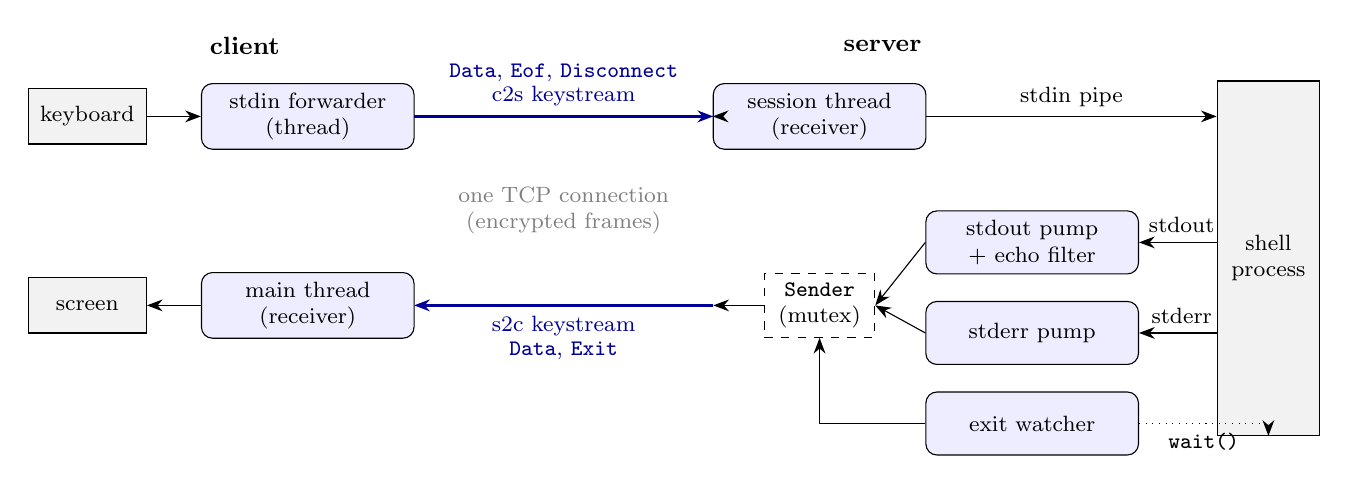
\begin{tikzpicture}[
  font=\footnotesize, >={Stealth[length=2mm]},
  th/.style={draw, rounded corners, fill=blue!7, align=center, minimum width=2.7cm, minimum height=0.8cm},
  io/.style={draw, align=center, minimum width=1.5cm, minimum height=0.7cm, fill=gray!10},
  lock/.style={draw, dashed, align=center, minimum width=1.4cm, minimum height=0.6cm},
]
  % client
  \node[font=\bfseries\small] at (0.6,2.1) {client};
  \node[io] (kbd) at (-1.4,1.2) {keyboard};
  \node[io] (scr) at (-1.4,-1.2) {screen};
  \node[th] (fwd) at (1.4,1.2) {stdin forwarder\\(thread)};
  \node[th] (cmain) at (1.4,-1.2) {main thread\\(receiver)};
  \draw[->] (kbd) -- (fwd);
  \draw[->] (cmain) -- (scr);

  % wire
  \draw[->, very thick, blue!60!black] (2.75,1.2) -- node[above, align=center]{\texttt{Data}, \texttt{Eof}, \texttt{Disconnect}\\[-1pt] c2s keystream} (6.55,1.2);
  \draw[<-, very thick, blue!60!black] (2.75,-1.2) -- node[below, align=center]{s2c keystream\\[-1pt] \texttt{Data}, \texttt{Exit}} (6.55,-1.2);
  \node[gray, align=center] at (4.65,0) {one TCP connection\\(encrypted frames)};

  % server
  \node[font=\bfseries\small] at (8.7,2.1) {server};
  \node[th] (sess) at (7.9,1.2) {session thread\\(receiver)};
  \node[lock] (snd) at (7.9,-1.2) {\texttt{Sender}\\ (mutex)};
  \node[th] (pout) at (10.6,-0.4) {stdout pump\\+ echo filter};
  \node[th] (perr) at (10.6,-1.55) {stderr pump};
  \node[th] (watch) at (10.6,-2.7) {exit watcher};
  \node[io, minimum height=4.5cm, minimum width=1.3cm] (sh) at (13.6,-0.6) {shell\\process};
  \draw[->] (sess) -- node[above]{stdin pipe} (sh.north west |- sess);
  \draw[<-] (pout) -- node[above, pos=0.55]{stdout} (pout -| sh.west);
  \draw[<-] (perr) -- node[above, pos=0.55]{stderr} (perr -| sh.west);
  \draw[->] (pout.west) -- (snd.east);
  \draw[->] (perr.west) -- (snd.east);
  \draw[->] (watch.west) -| (snd.south);
  \draw[->, dotted] (watch.east) -| node[pos=0.25, below]{\texttt{wait()}} (sh.south);
  \draw[->] (snd.west) -- (6.55,-1.2);
  \draw[<-] (sess.west) -- (6.55,1.2);
\end{tikzpicture}}
\caption{Threads of one interactive session. The three server threads that send share one \texttt{Sender} behind a mutex, so their messages never interleave inside a frame and the keystream positions stay in order.}
\label{fig:threads}
\end{figure}

The mutex around the \texttt{Sender} matters for the encryption: the cipher
state moves forward with every byte, so two threads must never encrypt at the
same time. Each frame is encrypted and written while the lock is held, which
makes the order of frames on the wire the same as the order of keystream use.

\Needspace{18\baselineskip}
\begin{lstlisting}[caption={The server's input loop (\texttt{server/shell.rs}).}]
let result = loop {
    match receiver.recv() {                         // decrypt with the c2s keystream
        Ok(Message::Data(data)) => {
            if let Some(input) = stdin.as_mut() {
                echo.lock().unwrap().expect(&data); // Windows: note the echo
                if input.write_all(&data).and_then(|_| input.flush()).is_err() {
                    stdin = None;                   // shell closed its input
                }
            }
        }
        Ok(Message::Eof) => stdin = None,           // dropping the pipe sends EOF
        Ok(Message::Disconnect) => break Ok(()),
        Ok(_) => break Err(invalid("unexpected message during shell")),
        Err(e) => break Err(e),                     // connection lost
    }
};
drop(stdin);
let _ = child.lock().unwrap().kill();               // never leave a shell behind
\end{lstlisting}

\textbf{How a session ends.} Every way out ends with the shell gone and the
client told why:

\begin{table}[H]
\centering
\footnotesize
\begin{tabularx}{\textwidth}{@{}l X@{}}
\toprule
Event & What happens \\
\midrule
User types \texttt{exit 3} & the shell exits; its pipes close, both pumps finish, the watcher collects code 3 and sends \texttt{Exit(3)}; the client sends \texttt{Disconnect} and exits with code 3 \\
End of input on the client (Ctrl+D, end of a pipe) & the forwarder sends \texttt{Eof}; the server drops the shell's stdin pipe; \texttt{sh} sees end of input and exits as above \\
Client killed or network lost & the server's \texttt{recv} fails, the loop ends and the server kills the shell \\
Shell killed on the server & it has no exit code; the watcher sends \texttt{Exit(-1)} \\
Shell cannot be started & the server sends \texttt{Failure("cannot start shell: \ldots")} instead of \texttt{Success} \\
\bottomrule
\end{tabularx}
\caption{Ending an interactive session.}
\end{table}

\textbf{Echo filter.} With no terminal attached, \texttt{cmd.exe} echoes every
command line it reads to its output, so the user would see each command twice.
On Windows the server therefore records each complete input line, for example
\texttt{dir\textbackslash r\textbackslash n}, and the stdout pump removes
exactly that byte sequence when it arrives. As soon as the output differs from
what was expected, the held bytes are released, so real output is never lost.
On other systems the filter does nothing, because \texttt{sh} does not echo.

\textbf{File copy.} \texttt{rcp} uses the same connection and handshake but
sends one \texttt{Upload} (path, file name, contents) or \texttt{Download}
(path) and waits for \texttt{Success}, \texttt{File} or \texttt{Failure},
then sends \texttt{Disconnect}. The whole file travels in one encrypted
message, so its contents are protected exactly like the shell traffic.


The output side is one \emph{pump} per pipe. Each sends what the shell printed
as a \texttt{Data} message, through the shared \texttt{Sender}:

\Needspace{17\baselineskip}
\begin{lstlisting}[caption={An output pump (\texttt{server/shell.rs}).}]
thread::spawn(move || {
    let mut buf = [0u8; 4096];
    loop {
        let n = match source.read(&mut buf) { Ok(0) | Err(_) => break, Ok(n) => n };
        let data = match &echo {
            Some(filter) => filter.lock().unwrap().filter(&buf[..n]),
            None => buf[..n].to_vec(),
        };
        if !data.is_empty() && sender.lock().unwrap().send(&Message::Data(data)).is_err() {
            return;                         // client is gone
        }
    }
})
\end{lstlisting}

\subsection{ARP server and client}

\Needspace{15\baselineskip}
\begin{lstlisting}[caption={Learning and answering in the ARP server loop (\texttt{server.rs}).}]
let request = match ArpPacket::decode(&buf[..n]) {
    Some(p) if p.op == REQUEST => p,
    _ => continue,                             // malformed or not a request
};
if table.insert(request.sender_ip, request.sender_mac).is_none() {
    println!("Learned {} is at {}", request.sender_ip, request.sender_mac);
}
match table.get(&request.target_ip) {
    Some(&mac) => { socket.send_to(&request.reply_to(mac).encode(), from)?; }
    None => println!("No host has {}, request dropped", request.target_ip),
}
\end{lstlisting}

The reply swaps the roles: the found MAC becomes the sender hardware address and
the requester becomes the target. The client keeps a
\texttt{BTreeMap<Ipv4Addr, (Mac, Instant)>} and drops entries older than 60\,s
before every lookup; a request that gets no matching reply within 2\,s is
reported as \texttt{No reply}.

% ---------------------------------------------------------------- 4
\section{Test Cases}
\label{sec:tests}

The projects had no tests, so three test files were added without changing the
programs. The rsh tests use the library crates directly; the handshake tests run
on real TCP connections on \texttt{127.0.0.1} through a small relay that keeps a
copy of every byte. The ARP tests start the real \texttt{arp} binary and talk to
it with packets built by hand from RFC~826, so they also check the wire format.

\begin{table}[H]
\centering
\footnotesize
\begin{tabularx}{\textwidth}{@{}>{\ttfamily\scriptsize}l X@{}}
\toprule
\normalfont Test & Input and expected result \\
\midrule
\multicolumn{2}{@{}l}{\textit{rsh-crypto/tests/crypto.rs}} \\
modular\_arithmetic\_is\_correct & 1000 random moduli: $ab \bmod m$ and $a \cdot a^{-1} \equiv 1$; no inverse when $\gcd \ne 1$ \\
miller\_rabin\_agrees\_with\_sieve & every $n \le 200\,000$ matches a sieve; Carmichael numbers rejected; $2^{61}-1$ and $2^{64}-59$ prime \\
keys\_have\_64\_bit\_modulus & 50 keys: $n \ge 2^{62}$, $e = 65537$, $(m^{e})^{d} \equiv m$ \\
rsa\_encrypt\_decrypt\_round\_trip & lengths 0--99 bytes: round trip, ciphertext is $4 + 8\lceil \ell/7 \rceil$ bytes \\
wrong\_private\_key\_cannot\_decrypt & another key gives other bytes; a cut ciphertext is an error \\
signatures\_verify\_and\_detect\_changes & wrong key, one changed data bit or signature bit: rejected \\
stream\_cipher\_round\_trip\_and\_directions & round trip; the two directions and two keys give different streams \\
flipped\_ciphertext\_bit\_flips\_plaintext\_bit & flipping wire bits turns \texttt{rm -i} into \texttt{rm -f} without the key \\
key\_files\_round\_trip & public and private key text formats round-trip; bad lines rejected \\
fingerprint\_format & 8 colon-separated hex bytes \\
\multicolumn{2}{@{}l}{\textit{rsh-crypto/tests/attack.rs}} \\
pollard\_rho\_finds\_factors & 140 moduli of 16--64 bits: a prime factor is found every time \\
public\_key\_alone\_recovers\_session\_key & 10 real keys: $d$ recovered, session key decrypted, signature forged \\
factoring\_time\_by\_modulus\_size & timing table for trial division and Pollard's rho (Table~\ref{tab:factor}) \\
\multicolumn{2}{@{}l}{\textit{rsh-main/tests/protocol.rs}} \\
every\_message\_round\_trips & all 13 message types encode and decode to the same value \\
malformed\_messages\_are\_rejected & empty, unknown tag, truncated, trailing byte, bad UTF-8: errors \\
frames\_round\_trip\_and\_enforce\_limits & two frames read back; length 0 and $> 64$\,MiB refused both ways \\
handshake\_then\_encrypted\_data & full login over TCP, data both ways; user name and command never on the wire \\
unknown\_client\_key\_is\_rejected & stranger key: \texttt{PermissionDenied}, ``not in authorized\_keys'' \\
changed\_host\_key\_is\_refused & same host name, new host key: ``HAS CHANGED'' \\
recorded\_login\_can\_be\_replayed & the two recorded login frames, sent again by a keyless client, are accepted \\
\multicolumn{2}{@{}l}{\textit{arp/tests/arp.rs}} \\
reply\_has\_rfc826\_layout & reply to a hand-built request equals the expected 28 bytes exactly \\
all\_preloaded\_hosts\_resolve & the four table entries give their MAC addresses \\
unknown\_host\_gets\_no\_reply & \texttt{192.168.1.99}: no datagram comes back \\
server\_learns\_the\_sender & unknown before, known after that host sends one request \\
malformed\_packets\_are\_ignored & wrong htype, ptype, hlen, a reply, 20 bytes, empty: no answer, server still up \\
any\_request\_can\_overwrite\_an\_entry & a request claiming \texttt{192.168.1.1} replaces the gateway's MAC \\
client\_uses\_its\_cache & client binary: one request for two lookups, \texttt{Cache hit}, cache table \\
second\_client\_finds\_the\_first & client B resolves client A's address; bad input reported \\
udp\_round\_trip\_time & 1000 request/reply round trips timed \\
\bottomrule
\end{tabularx}
\caption{Automated tests (29 in total).}
\end{table}

\Needspace{20\baselineskip}
All 29 tests pass (\texttt{cargo test -{}-workspace} in \texttt{rsh/}, \texttt{cargo test} in \texttt{arp/}):

\noindent\begin{minipage}[t]{0.495\textwidth}
\begin{lstlisting}[style=plain,basicstyle=\ttfamily\fontsize{6.4}{7.8}\selectfont]
test modular_arithmetic_is_correct ... ok
test miller_rabin_agrees_with_sieve ... ok
test keys_have_64_bit_modulus ... ok
test rsa_encrypt_decrypt_round_trip ... ok
test wrong_private_key_cannot_decrypt ... ok
test signatures_verify_and_detect_changes ... ok
test stream_cipher_round_trip_and_directions ... ok
test flipped_ciphertext_bit_flips_plaintext_bit ... ok
test key_files_round_trip ... ok
test fingerprint_format ... ok
test result: ok. 10 passed; 0 failed
test pollard_rho_finds_factors ... ok
test public_key_alone_recovers_session_key ... ok
test factoring_time_by_modulus_size ... ok
test result: ok. 3 passed; 0 failed
\end{lstlisting}
\end{minipage}\hfill
\begin{minipage}[t]{0.495\textwidth}
\begin{lstlisting}[style=plain,basicstyle=\ttfamily\fontsize{6.4}{7.8}\selectfont]
test every_message_round_trips ... ok
test malformed_messages_are_rejected ... ok
test frames_round_trip_and_enforce_limits ... ok
test handshake_then_encrypted_data ... ok
test unknown_client_key_is_rejected ... ok
test changed_host_key_is_refused ... ok
test recorded_login_can_be_replayed ... ok
test result: ok. 7 passed; 0 failed
test reply_has_rfc826_layout ... ok
test all_preloaded_hosts_resolve ... ok
test unknown_host_gets_no_reply ... ok
test server_learns_the_sender ... ok
test malformed_packets_are_ignored ... ok
test any_request_can_overwrite_an_entry ... ok
test client_uses_its_cache ... ok
test second_client_finds_the_first ... ok
test udp_round_trip_time ... ok
test result: ok. 9 passed; 0 failed
\end{lstlisting}
\end{minipage}

% ---------------------------------------------------------------- 5
\section{Results}

All measurements were taken on one Linux machine (4 cores, kernel 6.18, Rust
1.97, release build) over the loopback interface.

\subsection{Bytes on the wire}
\label{sec:wire}

Output of \texttt{handshake\_then\_encrypted\_data}. The relay split the
captured byte streams back into frames; sizes include the 4-byte length.

\begin{table}[H]
\centering
\small
\begin{tabularx}{\textwidth}{@{}l l r X@{}}
\toprule
Frame & Direction & Bytes & Make-up \\
\midrule
\texttt{HostKey}    & server $\to$ client & 21 & $4 + 1 + 8 + 8$, in clear \\
\texttt{SessionKey} & client $\to$ server & 53 & $4 + 1 + 4 + (4 + 5 \times 8)$: 32 key bytes in five RSA blocks \\
\texttt{Auth}       & client $\to$ server & 40 & $4 + 1 + (4 + 7) + 8 + 8 + 8$, user \texttt{student} \\
\texttt{Success}    & server $\to$ client & 24 & $4 + 1 + 4 + 15$, ``welcome student'' \\
\midrule
\multicolumn{2}{@{}l}{Whole login}   & 138 & 93 up, 45 down \\
\texttt{Data}, 20-byte command & client $\to$ server & 29 & 9 bytes of overhead per message \\
\bottomrule
\end{tabularx}
\caption{Frames of one login and one command.}
\label{tab:wire}
\end{table}

The test then searched the captured bytes. The command
\texttt{echo secret-command} and the user name \texttt{student} appear in
neither direction; only the host key and the RSA ciphertext of the session key
are readable on the wire.

\subsection{An ARP request and its reply}

A request from \texttt{192.168.1.100} for \texttt{192.168.1.20}, and the
server's answer, as captured by a small UDP client:

\begin{lstlisting}[style=plain]
request: 00 01 08 00 06 04 00 01 02 00 c0 a8 01 64 c0 a8 01 64 00 00 00 00 00 00 c0 a8 01 14
reply:   00 01 08 00 06 04 00 02 00 1a 2b 3c 4d 14 c0 a8 01 14 02 00 c0 a8 01 64 c0 a8 01 64
         <htype> <ptype> hl pl <oper> <---sender MAC--> <sender IP> <---target MAC--> <target IP>
\end{lstlisting}

The operation changed from 1 to 2, the found MAC \texttt{00:1a:2b:3c:4d:14}
and \texttt{192.168.1.20} moved to the sender fields, and the requester moved to
the target fields. A full request/reply round trip over loopback took
36.4\,\textmu s on average over 1000 rounds (\texttt{udp\_round\_trip\_time}).
An address that nobody knows costs the client its whole 2\,s timeout, because
the server sends nothing back.

\subsection{Breaking the 64-bit key}

\texttt{factoring\_time\_by\_modulus\_size} builds 20 moduli for each size from
two primes of half that size and factors them. Trial division was stopped at
48 bits.

\begin{table}[H]
\centering
\small
\begin{tabular}{@{}r r r@{}}
\toprule
Modulus bits & Trial division (ms) & Pollard's rho (ms) \\
\midrule
24 & 0.002  & 0.003 \\
32 & 0.035  & 0.006 \\
40 & 0.896  & 0.017 \\
48 & 14.558 & 0.063 \\
56 & --     & 0.160 \\
64 & --     & 1.018 \\
\bottomrule
\end{tabular}
\caption{Mean time to factor one modulus (20 moduli per row).}
\label{tab:factor}
\end{table}

\texttt{public\_key\_alone\_recovers\_session\_key} then attacked ten real
\texttt{KeyPair::generate} keys, using nothing but the public key. Each was
factored in 0.29--1.21\,ms (mean 0.85\,ms). In every case the recovered $d$ was
the real private exponent, it decrypted a 32-byte session key encrypted to that
host, and a signature made with it was accepted by \texttt{verify}.

\begin{figure}[H]
\centering
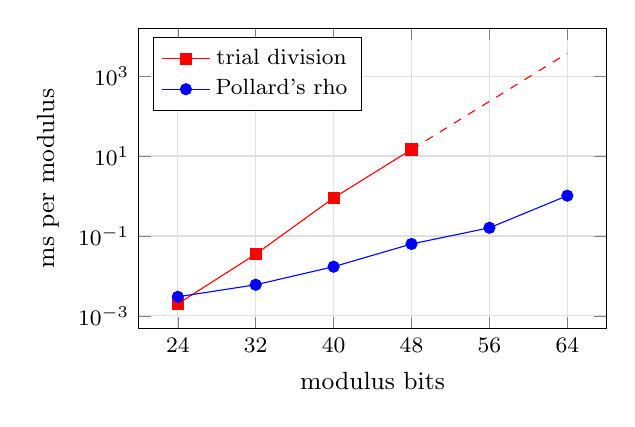
\begin{tikzpicture}
\begin{semilogyaxis}[
  width=0.62\textwidth, height=5.4cm,
  xlabel={modulus bits}, ylabel={ms per modulus},
  xtick={24,32,40,48,56,64},
  legend pos=north west, legend style={font=\footnotesize},
  grid=major, grid style={gray!25},
  tick label style={font=\footnotesize}, label style={font=\small},
]
\addplot[mark=square*,red] coordinates {(24,0.002) (32,0.035) (40,0.896) (48,14.558)};
\addplot[mark=*,blue] coordinates {(24,0.003) (32,0.006) (40,0.017) (48,0.063) (56,0.160) (64,1.018)};
\addplot[dashed,red,forget plot] coordinates {(48,14.558) (56,233) (64,3727)};
\legend{trial division, Pollard's rho}
\end{semilogyaxis}
\end{tikzpicture}
\caption{Factoring time against modulus size. The dashed line extends trial division by its measured growth of about $16\times$ per 8 bits.}
\label{fig:factor}
\end{figure}

\subsection{File copy time and the Nagle effect}
\label{sec:nagle}

Files of 1\,KB to 65\,000\,KB were copied five times in each direction with
\texttt{rcp}, and the median time it reported is shown (connection, handshake
and transfer). The first copies showed a floor of about 130\,ms even for one
kilobyte. To find the cause, the same tests were repeated with a copy of the
code in which \texttt{Transport::new} also calls
\texttt{stream.set\_nodelay(true)}, which turns off Nagle's algorithm. This
one-line change was only an experiment; it is not part of the submitted code.

\begin{table}[H]
\centering
\small
\begin{tabular}{@{}r r r r r@{}}
\toprule
& \multicolumn{2}{c}{as submitted} & \multicolumn{2}{c}{with \texttt{TCP\_NODELAY}} \\
\cmidrule(lr){2-3}\cmidrule(l){4-5}
File size (KB) & upload (ms) & download (ms) & upload (ms) & download (ms) \\
\midrule
1      & 129.9 & 131.6 & 0.75  & 0.57  \\
4      & 131.6 & 129.9 & 0.71  & 0.62  \\
16     & 130.0 & 130.0 & 0.85  & 0.87  \\
64     & 86.2  & 86.3  & 0.91  & 0.79  \\
256    & 85.9  & 89.7  & 1.69  & 1.31  \\
1024   & 89.6  & 89.8  & 3.86  & 4.47  \\
4096   & 100.0 & 101.4 & 13.76 & 13.47 \\
16384  & 144.0 & 144.4 & 59.6  & 57.1  \\
65000  & 324.8 & 372.6 & 288.9 & 280.3 \\
65536  & \multicolumn{4}{c}{\texttt{rcp: packet too large}} \\
\bottomrule
\end{tabular}
\caption{Median \texttt{rcp} time over loopback (5 runs per cell).}
\label{tab:rcp}
\end{table}

\begin{figure}[H]
\centering
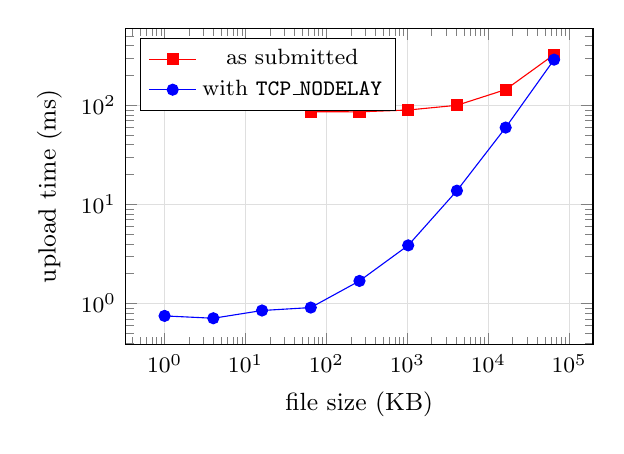
\begin{tikzpicture}
\begin{loglogaxis}[
  width=0.62\textwidth, height=5.6cm,
  xlabel={file size (KB)}, ylabel={upload time (ms)},
  legend pos=north west, legend style={font=\footnotesize},
  grid=major, grid style={gray!25},
  tick label style={font=\footnotesize}, label style={font=\small},
]
\addplot[mark=square*,red] coordinates {(1,129.9) (4,131.6) (16,130.0) (64,86.2) (256,85.9) (1024,89.6) (4096,100.0) (16384,144.0) (65000,324.8)};
\addplot[mark=*,blue] coordinates {(1,0.75) (4,0.71) (16,0.85) (64,0.91) (256,1.69) (1024,3.86) (4096,13.76) (16384,59.6) (65000,288.9)};
\legend{as submitted, with \texttt{TCP\_NODELAY}}
\end{loglogaxis}
\end{tikzpicture}
\caption{Upload time against file size.}
\label{fig:rcp}
\end{figure}

The same difference shows in an interactive login. Twenty runs of
\texttt{rsh connect} that type only \texttt{exit} took a median of 222.8\,ms
(221.1--227.1\,ms) as submitted and 3.5\,ms (3.4--5.3\,ms) with
\texttt{TCP\_NODELAY}, including process start-up and starting the remote shell.

\subsection{Live run}

One server and one client on the same machine, user \texttt{student}, empty
\texttt{RSH\_HOME} (long paths shortened). The shell is \texttt{sh -i}, which
prints its \texttt{\#} prompt on standard error.

\begin{lstlisting}[style=plain]
$ rsh-keygen -a
The key fingerprint is:
6b:d4:0f:0f:c2:ab:f5:a2 student@labpc
Modulus n = 8775609486456326389 (64-bit), e = 65537
Added key to $RSH_HOME/authorized_keys

$ rsh connect 127.0.0.1
# typed: whoami | GREETING=hello; echo $GREETING | cd /tmp && pwd | ls /nonexistent | exit 3
Host '127.0.0.1:2222' is not known. Key fingerprint is ca:08:8a:d8:51:e2:89:5c.
Warning: Permanently added '127.0.0.1:2222' to the list of known hosts.
Connected to 127.0.0.1:2222. Type 'exit' to leave.
sh: 0: can't access tty; job control turned off
# root
# # hello
/tmp
# ls: cannot access '/nonexistent': No such file or directory
# Connection to 127.0.0.1 closed.               (rsh exit code 3)

$ rcp notes.txt 127.0.0.1:backup.txt
backup.txt                     100%         32 bytes       0.2 KB/s   0.13s
$ rcp 127.0.0.1:missing.txt x.txt
rcp: missing.txt: No such file or directory (os error 2)
$ RSH_HOME=other rsh connect 127.0.0.1           # a key that is not authorized
rsh: authentication failed: key 8e:d9:16:5a:ee:82:4c:94 is not in authorized_keys
$ rsh connect 127.0.0.1                          # after the server made a new host key
rsh: HOST KEY FOR 127.0.0.1:2222 HAS CHANGED (now d2:56:47:b2:18:09:6d:30). Remove its line ...
\end{lstlisting}

Server log for the same run:

\begin{lstlisting}[style=plain]
Host key fingerprint: ca:08:8a:d8:51:e2:89:5c
rsh server listening on port 2222
[127.0.0.1:33428] connected
[127.0.0.1:33428] authenticated as student
[127.0.0.1:33428] shell started (pid 5399)
[127.0.0.1:33428] shell exited with code 3
[127.0.0.1:33428] disconnected
[127.0.0.1:33446] upload notes.txt -> backup.txt: Success("wrote 32 bytes to srv/backup.txt")
[127.0.0.1:33458] download missing.txt
[127.0.0.1:33474] closed: key 8e:d9:16:5a:ee:82:4c:94 is not in authorized_keys
[127.0.0.1:33480] closed: failed to fill whole buffer          (client hung up after the host key)
\end{lstlisting}

The ARP server with two clients. Client A (\texttt{192.168.1.100}) looked up
\texttt{.10} twice and \texttt{.99} once; client B (\texttt{192.168.1.101}) then
looked up client A. Server log:

\begin{lstlisting}[style=plain]
127.0.0.1:47232 -> ARP Request: who has 192.168.1.10? tell 192.168.1.100 (02:00:c0:a8:01:64)
Learned 192.168.1.100 is at 02:00:c0:a8:01:64
127.0.0.1:47232 <- ARP Reply: 192.168.1.10 is at 00:1a:2b:3c:4d:0a
127.0.0.1:47232 -> ARP Request: who has 192.168.1.99? tell 192.168.1.100 (02:00:c0:a8:01:64)
No host has 192.168.1.99, request dropped
127.0.0.1:49944 -> ARP Request: who has 192.168.1.100? tell 192.168.1.101 (02:00:c0:a8:01:65)
Learned 192.168.1.101 is at 02:00:c0:a8:01:65
127.0.0.1:49944 <- ARP Reply: 192.168.1.100 is at 02:00:c0:a8:01:64
\end{lstlisting}

Client A printed \texttt{Cache hit} for its second lookup of \texttt{.10},
which sent nothing (the server log shows only one request), \texttt{No reply}
for \texttt{.99}, and a cache table with \texttt{.10} expiring in 57\,s. Client B
received A's MAC address, which the server had only learned from A's request.

% ---------------------------------------------------------------- 6
\section{Observations}

\begin{enumerate}
\item \textbf{The handshake does its job.} A new host key is remembered, a
  changed one is refused, and a client key that is not in
  \texttt{authorized\_keys} is turned away, both in the tests and in the live
  run. A login costs 138 bytes and every later message 9 bytes of overhead.

\item \textbf{Everything after the session key is hidden.} Neither the user name
  nor the typed command appears in the captured traffic. Only the host key and
  the RSA-encrypted session key travel in clear.

\item \textbf{A 64-bit key is not a secret.} Pollard's rho factored every real
  host key in about a millisecond, which gives the private key and with it the
  session key and the whole recorded session. Its cost grows roughly as
  $n^{1/4}$, about $4\times$ per 8 bits, while trial division grows as
  $n^{1/2}$, about $16\times$ per 8 bits (Table~\ref{tab:factor}). Even trial
  division would need only a few seconds at 64 bits.

\item \textbf{Encryption without integrity can be changed and replayed.}
  Flipping ciphertext bits flips the same plaintext bits, so \texttt{rm -i}
  became \texttt{rm -f} without knowing the key. Because the client alone
  chooses the session key and the server adds nothing random, a recorded login
  can be sent again and is accepted. The attacker cannot read the replayed
  session, but the server runs it.

\item \textbf{Small messages wait for TCP, not for the network.} Every frame is
  written as two \texttt{write} calls, a 4-byte length and then the body. With
  Nagle's algorithm on, the second small segment waits for the ACK of the first,
  and the receiver delays that ACK by about 40\,ms. Files up to 16\,KB took
  $\approx 130\text{ ms} \approx 3 \times 43$\,ms; from 64\,KB, where the body is
  larger than one loopback segment and goes out at once, they took
  $\approx 86\text{ ms} \approx 2 \times 43$\,ms. With \texttt{TCP\_NODELAY}
  a 1\,KB copy took 0.75\,ms and a login 3.5\,ms instead of 223\,ms, about
  $64\times$ faster. Large files are limited by copying, about 200\,MB/s either
  way.

\item \textbf{Encryption costs size only in the framing.} Typing
  \texttt{whoami} sent 8 readable bytes over Telnet
  (\texttt{whoami\textbackslash r\textbackslash n}) and a 16-byte frame over
  rsh: the stream cipher adds no bytes at all, and the 9 extra bytes are the
  frame length, the message tag and the field length.

\item \textbf{One message per file sets a size limit.} A 65\,000\,KB file was
  copied, but a 64\,MiB file fails with \texttt{packet too large}, because the
  whole file must fit in one frame.

\item \textbf{ARP trusts whatever it hears.} Learning from requests lets client
  B find client A without any configuration, which is the point of ARP. The same
  rule lets any host claim \texttt{192.168.1.1} and redirect the gateway to
  itself (\texttt{any\_request\_can\_overwrite\_an\_entry}), which is exactly
  ARP spoofing. The cache turns a repeated lookup into no traffic at all, and
  matters most for a missing host, where a miss costs the full 2\,s timeout.
\end{enumerate}

% ---------------------------------------------------------------- 7
\section{Possible Improvements}

\begin{itemize}
\item Write the length and the body of a frame in one \texttt{write} call, or
  set \texttt{TCP\_NODELAY}. Section~\ref{sec:nagle} shows this removes 40\,ms stalls and
  makes a login about $64\times$ faster.
\item Let the server send a random nonce with its host key and have the client
  sign it as well, so that a recorded login cannot be replayed.
\item Add a message authentication code with a sequence number to every frame,
  so that changed, dropped or reordered messages are detected.
\item Use larger keys (2048-bit RSA) with padding, a real hash and a real
  cipher. The random generator should also be seeded with more than 64 bits.
\item \texttt{rcp} writes a downloaded file to \texttt{local/<name>} with the name
  the server sends. A malicious server could send \texttt{../../.bashrc}; the
  client should accept a plain file name only, as the server already does for
  uploads. Private key files should be created with mode \texttt{0600}.
\item Send files in chunks instead of one message, which removes the 64\,MiB
  limit and the need to hold the whole file in memory.
\item Give the remote shell a pseudo-terminal, so that full-screen programs and
  Ctrl+C work.
\item In ARP, keep the preloaded entries static and log when a learned address
  changes its MAC, which is how ARP spoofing is usually noticed.
\end{itemize}

% ---------------------------------------------------------------- 8
\section{Comments}

Starting with Telnet and then securing it made the purpose of each part of
SSH concrete: the recorded Telnet session showed the password on the wire, and
the same kind of session over rsh showed only noise, with each piece of the
cryptography accounting for one of the missing guarantees. Building both
protocols from the standard library alone made every layer visible: the bytes of an ARP packet, the length prefix of a frame, the RSA
arithmetic and the order of the handshake messages. The tests showed that the
design is right in structure, since host keys, authorized keys and encryption
all behave as intended, but also why real protocols carry more than this: a key
that can be factored in a millisecond, a session that can be replayed, and
ciphertext that can be changed. The most surprising result was not about
security at all. A small detail of how a frame is written, two writes instead
of one, made every login 64 times slower, which only showed up once the
programs were measured.

\end{document}
